\documentclass[1p]{elsarticle_modified}
%\bibliographystyle{elsarticle-num}

%\usepackage[colorlinks]{hyperref}
%\usepackage{abbrmath_seonhwa} %\Abb, \Ascr, \Acal ,\Abf, \Afrak
\usepackage{amsfonts}
\usepackage{amssymb}
\usepackage{amsmath}
\usepackage{amsthm}
\usepackage{scalefnt}
\usepackage{amsbsy}
\usepackage{kotex}
\usepackage{caption}
\usepackage{subfig}
\usepackage{color}
\usepackage{graphicx}
\usepackage{xcolor} %% white, black, red, green, blue, cyan, magenta, yellow
\usepackage{float}
\usepackage{setspace}
\usepackage{hyperref}

\usepackage{tikz}
\usetikzlibrary{arrows}

\usepackage{multirow}
\usepackage{array} % fixed length table
\usepackage{hhline}

%%%%%%%%%%%%%%%%%%%%%
\makeatletter
\renewcommand*\env@matrix[1][\arraystretch]{%
	\edef\arraystretch{#1}%
	\hskip -\arraycolsep
	\let\@ifnextchar\new@ifnextchar
	\array{*\c@MaxMatrixCols c}}
\makeatother %https://tex.stackexchange.com/questions/14071/how-can-i-increase-the-line-spacing-in-a-matrix
%%%%%%%%%%%%%%%

\usepackage[normalem]{ulem}

\newcommand{\msout}[1]{\ifmmode\text{\sout{\ensuremath{#1}}}\else\sout{#1}\fi}
%SOURCE: \msout is \stkout macro in https://tex.stackexchange.com/questions/20609/strikeout-in-math-mode

\newcommand{\cancel}[1]{
	\ifmmode
	{\color{red}\msout{#1}}
	\else
	{\color{red}\sout{#1}}
	\fi
}

\newcommand{\add}[1]{
	{\color{blue}\uwave{#1}}
}

\newcommand{\replace}[2]{
	\ifmmode
	{\color{red}\msout{#1}}{\color{blue}\uwave{#2}}
	\else
	{\color{red}\sout{#1}}{\color{blue}\uwave{#2}}
	\fi
}

\newcommand{\Sol}{\mathcal{S}} %segment
\newcommand{\D}{D} %diagram
\newcommand{\A}{\mathcal{A}} %arc


%%%%%%%%%%%%%%%%%%%%%%%%%%%%%5 test

\def\sl{\operatorname{\textup{SL}}(2,\Cbb)}
\def\psl{\operatorname{\textup{PSL}}(2,\Cbb)}
\def\quan{\mkern 1mu \triangleright \mkern 1mu}

\theoremstyle{definition}
\newtheorem{thm}{Theorem}[section]
\newtheorem{prop}[thm]{Proposition}
\newtheorem{lem}[thm]{Lemma}
\newtheorem{ques}[thm]{Question}
\newtheorem{cor}[thm]{Corollary}
\newtheorem{defn}[thm]{Definition}
\newtheorem{exam}[thm]{Example}
\newtheorem{rmk}[thm]{Remark}
\newtheorem{alg}[thm]{Algorithm}

\newcommand{\I}{\sqrt{-1}}
\begin{document}

%\begin{frontmatter}
%
%\title{Boundary parabolic representations of knots up to 8 crossings}
%
%%% Group authors per affiliation:
%\author{Yunhi Cho} 
%\address{Department of Mathematics, University of Seoul, Seoul, Korea}
%\ead{yhcho@uos.ac.kr}
%
%
%\author{Seonhwa Kim} %\fnref{s_kim}}
%\address{Center for Geometry and Physics, Institute for Basic Science, Pohang, 37673, Korea}
%\ead{ryeona17@ibs.re.kr}
%
%\author{Hyuk Kim}
%\address{Department of Mathematical Sciences, Seoul National University, Seoul 08826, Korea}
%\ead{hyukkim@snu.ac.kr}
%
%\author{Seokbeom Yoon}
%\address{Department of Mathematical Sciences, Seoul National University, Seoul, 08826,  Korea}
%\ead{sbyoon15@snu.ac.kr}
%
%\begin{abstract}
%We find all boundary parabolic representation of knots up to 8 crossings.
%
%\end{abstract}
%\begin{keyword}
%    \MSC[2010] 57M25 
%\end{keyword}
%
%\end{frontmatter}

%\linenumbers
%\tableofcontents
%
\newcommand\colored[1]{\textcolor{white}{\rule[-0.35ex]{0.8em}{1.4ex}}\kern-0.8em\color{red} #1}%
%\newcommand\colored[1]{\textcolor{white}{ #1}\kern-2.17ex	\textcolor{white}{ #1}\kern-1.81ex	\textcolor{white}{ #1}\kern-2.15ex\color{red}#1	}

{\Large $\underline{12a_{1156}~(K12a_{1156})}$}

\setlength{\tabcolsep}{10pt}
\renewcommand{\arraystretch}{1.6}
\vspace{1cm}\begin{tabular}{m{100pt}>{\centering\arraybackslash}m{274pt}}
\multirow{5}{120pt}{
	\centering
	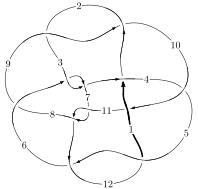
\includegraphics[width=112pt]{../../../GIT/diagram.site/Diagrams/png/1957_12a_1156.png}\\
\ \ \ A knot diagram\footnotemark}&
\allowdisplaybreaks
\textbf{Linearized knot diagam} \\
\cline{2-2}
 &
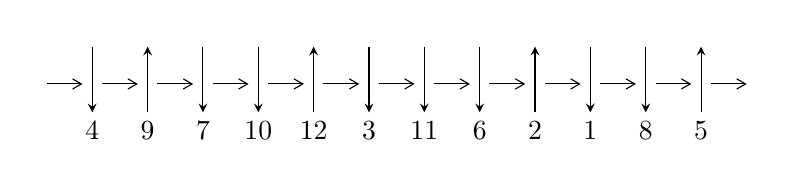
\begin{tikzpicture}[x=20pt, y=17pt]
	% nodes
	\node (C0) at (0, 0) {};
	\node (C1) at (1, 0) {};
	\node (C1U) at (1, +1) {};
	\node (C1D) at (1, -1) {4};

	\node (C2) at (2, 0) {};
	\node (C2U) at (2, +1) {};
	\node (C2D) at (2, -1) {9};

	\node (C3) at (3, 0) {};
	\node (C3U) at (3, +1) {};
	\node (C3D) at (3, -1) {7};

	\node (C4) at (4, 0) {};
	\node (C4U) at (4, +1) {};
	\node (C4D) at (4, -1) {10};

	\node (C5) at (5, 0) {};
	\node (C5U) at (5, +1) {};
	\node (C5D) at (5, -1) {12};

	\node (C6) at (6, 0) {};
	\node (C6U) at (6, +1) {};
	\node (C6D) at (6, -1) {3};

	\node (C7) at (7, 0) {};
	\node (C7U) at (7, +1) {};
	\node (C7D) at (7, -1) {11};

	\node (C8) at (8, 0) {};
	\node (C8U) at (8, +1) {};
	\node (C8D) at (8, -1) {6};

	\node (C9) at (9, 0) {};
	\node (C9U) at (9, +1) {};
	\node (C9D) at (9, -1) {2};

	\node (C10) at (10, 0) {};
	\node (C10U) at (10, +1) {};
	\node (C10D) at (10, -1) {1};

	\node (C11) at (11, 0) {};
	\node (C11U) at (11, +1) {};
	\node (C11D) at (11, -1) {8};

	\node (C12) at (12, 0) {};
	\node (C12U) at (12, +1) {};
	\node (C12D) at (12, -1) {5};
	\node (C13) at (13, 0) {};

	% arrows
	\draw[->,>={angle 60}]
	(C0) edge (C1) (C1) edge (C2) (C2) edge (C3) (C3) edge (C4) (C4) edge (C5) (C5) edge (C6) (C6) edge (C7) (C7) edge (C8) (C8) edge (C9) (C9) edge (C10) (C10) edge (C11) (C11) edge (C12) (C12) edge (C13) ;	\draw[->,>=stealth]
	(C1U) edge (C1D) (C2D) edge (C2U) (C3U) edge (C3D) (C4U) edge (C4D) (C5D) edge (C5U) (C6U) edge (C6D) (C7U) edge (C7D) (C8U) edge (C8D) (C9D) edge (C9U) (C10U) edge (C10D) (C11U) edge (C11D) (C12D) edge (C12U) ;
	\end{tikzpicture} \\
\hhline{~~} \\& 
\textbf{Solving Sequence} \\ \cline{2-2} 
 &
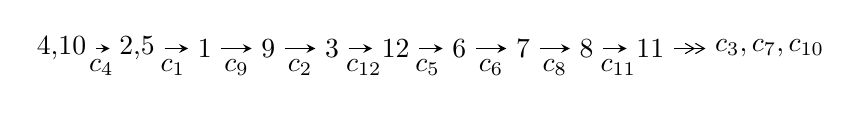
\begin{tikzpicture}[x=23pt, y=7pt]
	% node
	\node (A0) at (-1/8, 0) {4,10};
	\node (A1) at (17/16, 0) {2,5};
	\node (A2) at (17/8, 0) {1};
	\node (A3) at (25/8, 0) {9};
	\node (A4) at (33/8, 0) {3};
	\node (A5) at (41/8, 0) {12};
	\node (A6) at (49/8, 0) {6};
	\node (A7) at (57/8, 0) {7};
	\node (A8) at (65/8, 0) {8};
	\node (A9) at (73/8, 0) {11};
	\node (C1) at (1/2, -1) {$c_{4}$};
	\node (C2) at (13/8, -1) {$c_{1}$};
	\node (C3) at (21/8, -1) {$c_{9}$};
	\node (C4) at (29/8, -1) {$c_{2}$};
	\node (C5) at (37/8, -1) {$c_{12}$};
	\node (C6) at (45/8, -1) {$c_{5}$};
	\node (C7) at (53/8, -1) {$c_{6}$};
	\node (C8) at (61/8, -1) {$c_{8}$};
	\node (C9) at (69/8, -1) {$c_{11}$};
	\node (A10) at (11, 0) {$c_{3},c_{7},c_{10}$};

	% edge
	\draw[->,>=stealth]	
	(A0) edge (A1) (A1) edge (A2) (A2) edge (A3) (A3) edge (A4) (A4) edge (A5) (A5) edge (A6) (A6) edge (A7) (A7) edge (A8) (A8) edge (A9) ;
	\draw[->>,>={angle 60}]	
	(A9) edge (A10);
\end{tikzpicture} \\ 

\end{tabular} \\

\footnotetext{
The image of knot diagram is generated by the software ``\textbf{Draw programme}" developed by Andrew Bartholomew(\url{http://www.layer8.co.uk/maths/draw/index.htm\#Running-draw}), where we modified some parts for our purpose(\url{https://github.com/CATsTAILs/LinksPainter}).
}\phantom \\ \newline 
\centering \textbf{Ideals for irreducible components\footnotemark of $X_{\text{par}}$} 
 
\begin{align*}
I^u_{1}&=\langle 
-4.39785\times10^{29} u^{28}+7.02003\times10^{30} u^{27}+\cdots+4.21410\times10^{28} b+1.41325\times10^{31},\\
\phantom{I^u_{1}}&\phantom{= \langle  }5.66571\times10^{29} u^{28}-1.06111\times10^{31} u^{27}+\cdots+5.05693\times10^{29} a-3.29177\times10^{31},\\
\phantom{I^u_{1}}&\phantom{= \langle  }4 u^{29}-67 u^{28}+\cdots-1032 u+144\rangle \\
I^u_{2}&=\langle 
4.09097\times10^{106} a u^{58}-8.30494\times10^{109} u^{58}+\cdots+1.51366\times10^{108} a-4.79521\times10^{111},\\
\phantom{I^u_{2}}&\phantom{= \langle  }3.55453\times10^{112} a u^{58}-1.91263\times10^{111} u^{58}+\cdots+1.93423\times10^{114} a+1.37454\times10^{113},\\
\phantom{I^u_{2}}&\phantom{= \langle  }u^{59}+5 u^{58}+\cdots+88 u+37\rangle \\
I^u_{3}&=\langle 
-32 u^6+108 u^5-177 u^4+170 u^3-77 u^2+11 b-6 u+16,\\
\phantom{I^u_{3}}&\phantom{= \langle  }96 u^6-412 u^5+861 u^4-1115 u^3+935 u^2+11 a-455 u+106,\\
\phantom{I^u_{3}}&\phantom{= \langle  }4 u^7-17 u^6+36 u^5-48 u^4+43 u^3-24 u^2+8 u-1\rangle \\
I^u_{4}&=\langle 
-8148149 u^{18} a-235125959 u^{18}+\cdots+8148149 a+240741869,\\
\phantom{I^u_{4}}&\phantom{= \langle  }7782798 u^{18} a+171992551 u^{18}+\cdots+92850756 a-39782144,\;u^{19}+5 u^{18}+\cdots-4 u-1\rangle \\
\\
\end{align*}
\raggedright * 4 irreducible components of $\dim_{\mathbb{C}}=0$, with total 192 representations.\\
\footnotetext{All coefficients of polynomials are rational numbers. But the coefficients are sometimes approximated in decimal forms when there is not enough margin.}
\newpage
\renewcommand{\arraystretch}{1}
\centering \section*{I. $I^u_{1}= \langle -4.40\times10^{29} u^{28}+7.02\times10^{30} u^{27}+\cdots+4.21\times10^{28} b+1.41\times10^{31},\;5.67\times10^{29} u^{28}-1.06\times10^{31} u^{27}+\cdots+5.06\times10^{29} a-3.29\times10^{31},\;4 u^{29}-67 u^{28}+\cdots-1032 u+144 \rangle$}
\flushleft \textbf{(i) Arc colorings}\\
\begin{tabular}{m{7pt} m{180pt} m{7pt} m{180pt} }
\flushright $a_{4}=$&$\begin{pmatrix}1\\0\end{pmatrix}$ \\
\flushright $a_{10}=$&$\begin{pmatrix}0\\u\end{pmatrix}$ \\
\flushright $a_{2}=$&$\begin{pmatrix}-1.12039 u^{28}+20.9833 u^{27}+\cdots-489.650 u+65.0942\\10.4360 u^{28}-166.584 u^{27}+\cdots+2133.17 u-335.363\end{pmatrix}$ \\
\flushright $a_{5}=$&$\begin{pmatrix}1\\u^2\end{pmatrix}$ \\
\flushright $a_{1}=$&$\begin{pmatrix}9.31564 u^{28}-145.601 u^{27}+\cdots+1643.52 u-270.269\\10.4360 u^{28}-166.584 u^{27}+\cdots+2133.17 u-335.363\end{pmatrix}$ \\
\flushright $a_{9}=$&$\begin{pmatrix}-0.167275 u^{28}+1.19205 u^{27}+\cdots+351.772 u-65.4652\\-1.14188 u^{28}+19.5944 u^{27}+\cdots-355.098 u+47.1296\end{pmatrix}$ \\
\flushright $a_{3}=$&$\begin{pmatrix}-5.90644 u^{28}+97.0033 u^{27}+\cdots-1411.96 u+203.811\\9.23677 u^{28}-145.692 u^{27}+\cdots+1725.62 u-266.262\end{pmatrix}$ \\
\flushright $a_{12}=$&$\begin{pmatrix}7.09885 u^{28}-114.752 u^{27}+\cdots+1867.48 u-310.603\\2.01104 u^{28}-31.9469 u^{27}+\cdots+592.051 u-109.188\end{pmatrix}$ \\
\flushright $a_{6}=$&$\begin{pmatrix}0.300652 u^{28}-4.39629 u^{27}+\cdots+104.297 u-23.3575\\-0.314456 u^{28}+5.41479 u^{27}+\cdots+45.5803 u-17.0050\end{pmatrix}$ \\
\flushright $a_{7}=$&$\begin{pmatrix}-6.39600 u^{28}+102.252 u^{27}+\cdots-1202.06 u+178.195\\-3.56491 u^{28}+61.8556 u^{27}+\cdots-1702.73 u+287.027\end{pmatrix}$ \\
\flushright $a_{8}=$&$\begin{pmatrix}7.43460 u^{28}-120.183 u^{27}+\cdots+2485.47 u-437.881\\5.17344 u^{28}-80.0547 u^{27}+\cdots+1078.28 u-196.079\end{pmatrix}$ \\
\flushright $a_{11}=$&$\begin{pmatrix}10.9183 u^{28}-170.654 u^{27}+\cdots+2401.20 u-411.393\\12.2274 u^{28}-191.440 u^{27}+\cdots+2406.52 u-393.058\end{pmatrix}$\\&\end{tabular}
\flushleft \textbf{(ii) Obstruction class $= -1$}\\~\\
\flushleft \textbf{(iii) Cusp Shapes $= -56.3204 u^{28}+888.787 u^{27}+\cdots-10030.5 u+1517.92$}\\~\\
\newpage\renewcommand{\arraystretch}{1}
\flushleft \textbf{(iv) u-Polynomials at the component}\newline \\
\begin{tabular}{m{50pt}|m{274pt}}
Crossings & \hspace{64pt}u-Polynomials at each crossing \\
\hline $$\begin{aligned}c_{1},c_{10}\end{aligned}$$&$\begin{aligned}
&u^{29}+2 u^{27}+\cdots+13 u+4
\end{aligned}$\\
\hline $$\begin{aligned}c_{2},c_{5},c_{9}\\c_{12}\end{aligned}$$&$\begin{aligned}
&u^{29}+13 u^{27}+\cdots+3 u+1
\end{aligned}$\\
\hline $$\begin{aligned}c_{3},c_{6},c_{7}\\c_{11}\end{aligned}$$&$\begin{aligned}
&2(2 u^{29}+u^{28}+\cdots-2 u^2+1)
\end{aligned}$\\
\hline $$\begin{aligned}c_{4}\end{aligned}$$&$\begin{aligned}
&4(4 u^{29}-67 u^{28}+\cdots-1032 u+144)
\end{aligned}$\\
\hline $$\begin{aligned}c_{8}\end{aligned}$$&$\begin{aligned}
&u^{29}-9 u^{28}+\cdots-2794 u+324
\end{aligned}$\\
\hline
\end{tabular}\\~\\
\newpage\renewcommand{\arraystretch}{1}
\flushleft \textbf{(v) Riley Polynomials at the component}\newline \\
\begin{tabular}{m{50pt}|m{274pt}}
Crossings & \hspace{64pt}Riley Polynomials at each crossing \\
\hline $$\begin{aligned}c_{1},c_{10}\end{aligned}$$&$\begin{aligned}
&y^{29}+4 y^{28}+\cdots+361 y-16
\end{aligned}$\\
\hline $$\begin{aligned}c_{2},c_{5},c_{9}\\c_{12}\end{aligned}$$&$\begin{aligned}
&y^{29}+26 y^{28}+\cdots- y-1
\end{aligned}$\\
\hline $$\begin{aligned}c_{3},c_{6},c_{7}\\c_{11}\end{aligned}$$&$\begin{aligned}
&4(4 y^{29}-69 y^{28}+\cdots+4 y-1)
\end{aligned}$\\
\hline $$\begin{aligned}c_{4}\end{aligned}$$&$\begin{aligned}
&16(16 y^{29}-113 y^{28}+\cdots+197280 y-20736)
\end{aligned}$\\
\hline $$\begin{aligned}c_{8}\end{aligned}$$&$\begin{aligned}
&y^{29}-7 y^{28}+\cdots+371932 y-104976
\end{aligned}$\\
\hline
\end{tabular}\\~\\
\newpage\flushleft \textbf{(vi) Complex Volumes and Cusp Shapes}
$$\begin{array}{c|c|c}  
\text{Solutions to }I^u_{1}& \I (\text{vol} + \sqrt{-1}CS) & \text{Cusp shape}\\
 \hline 
\begin{aligned}
u &= \phantom{-}0.720097 + 0.708724 I \\
a &= \phantom{-}0.816159 - 0.207612 I \\
b &= -0.169307 + 1.103730 I\end{aligned}
 & -2.35305 + 2.75713 I & -6.94256 - 4.42813 I \\ \hline\begin{aligned}
u &= \phantom{-}0.720097 - 0.708724 I \\
a &= \phantom{-}0.816159 + 0.207612 I \\
b &= -0.169307 - 1.103730 I\end{aligned}
 & -2.35305 - 2.75713 I & -6.94256 + 4.42813 I \\ \hline\begin{aligned}
u &= -1.073600 + 0.143769 I \\
a &= -0.29269 + 1.43804 I \\
b &= \phantom{-}0.104360 - 0.757596 I\end{aligned}
 & -11.29210 - 3.08774 I & -16.1022 + 0.5651 I \\ \hline\begin{aligned}
u &= -1.073600 - 0.143769 I \\
a &= -0.29269 - 1.43804 I \\
b &= \phantom{-}0.104360 + 0.757596 I\end{aligned}
 & -11.29210 + 3.08774 I & -16.1022 - 0.5651 I \\ \hline\begin{aligned}
u &= \phantom{-}0.824430 + 0.723434 I \\
a &= -0.409830 + 0.858684 I \\
b &= -0.840941 - 1.121640 I\end{aligned}
 & -2.53290 - 7.99007 I & -6.91156 + 8.81648 I \\ \hline\begin{aligned}
u &= \phantom{-}0.824430 - 0.723434 I \\
a &= -0.409830 - 0.858684 I \\
b &= -0.840941 + 1.121640 I\end{aligned}
 & -2.53290 + 7.99007 I & -6.91156 - 8.81648 I \\ \hline\begin{aligned}
u &= \phantom{-}0.466322 + 0.746390 I \\
a &= \phantom{-}0.521683 - 0.597880 I \\
b &= \phantom{-}0.339053 + 0.681385 I\end{aligned}
 & \phantom{-}2.29372 + 0.20351 I & \phantom{-}3.05461 - 1.89825 I \\ \hline\begin{aligned}
u &= \phantom{-}0.466322 - 0.746390 I \\
a &= \phantom{-}0.521683 + 0.597880 I \\
b &= \phantom{-}0.339053 - 0.681385 I\end{aligned}
 & \phantom{-}2.29372 - 0.20351 I & \phantom{-}3.05461 + 1.89825 I \\ \hline\begin{aligned}
u &= \phantom{-}0.658708 + 0.957825 I \\
a &= -0.745982 - 0.471011 I \\
b &= \phantom{-}0.936085 - 0.375554 I\end{aligned}
 & -5.81070 + 3.60180 I & -14.0003 - 4.5219 I \\ \hline\begin{aligned}
u &= \phantom{-}0.658708 - 0.957825 I \\
a &= -0.745982 + 0.471011 I \\
b &= \phantom{-}0.936085 + 0.375554 I\end{aligned}
 & -5.81070 - 3.60180 I & -14.0003 + 4.5219 I\\
 \hline 
 \end{array}$$\newpage$$\begin{array}{c|c|c}  
\text{Solutions to }I^u_{1}& \I (\text{vol} + \sqrt{-1}CS) & \text{Cusp shape}\\
 \hline 
\begin{aligned}
u &= -0.057443 + 0.816735 I \\
a &= \phantom{-}0.837762 - 0.521934 I \\
b &= -0.102754 + 0.596050 I\end{aligned}
 & \phantom{-}0.31369 + 1.71075 I & \phantom{-}0.74020 - 4.40719 I \\ \hline\begin{aligned}
u &= -0.057443 - 0.816735 I \\
a &= \phantom{-}0.837762 + 0.521934 I \\
b &= -0.102754 - 0.596050 I\end{aligned}
 & \phantom{-}0.31369 - 1.71075 I & \phantom{-}0.74020 + 4.40719 I \\ \hline\begin{aligned}
u &= \phantom{-}0.745889 + 0.082585 I \\
a &= -0.150710 + 0.499245 I \\
b &= -0.96323 + 1.10340 I\end{aligned}
 & -1.67729 + 3.70537 I & -2.81014 - 3.47039 I \\ \hline\begin{aligned}
u &= \phantom{-}0.745889 - 0.082585 I \\
a &= -0.150710 - 0.499245 I \\
b &= -0.96323 - 1.10340 I\end{aligned}
 & -1.67729 - 3.70537 I & -2.81014 + 3.47039 I \\ \hline\begin{aligned}
u &= \phantom{-}1.086530 + 0.685326 I \\
a &= -0.229661 - 0.935105 I \\
b &= \phantom{-}1.61437 + 0.77483 I\end{aligned}
 & -7.32559 - 9.58865 I & \phantom{-0.000000 } 0 \\ \hline\begin{aligned}
u &= \phantom{-}1.086530 - 0.685326 I \\
a &= -0.229661 + 0.935105 I \\
b &= \phantom{-}1.61437 - 0.77483 I\end{aligned}
 & -7.32559 + 9.58865 I & \phantom{-0.000000 } 0 \\ \hline\begin{aligned}
u &= \phantom{-}1.222990 + 0.529637 I \\
a &= \phantom{-}0.003013 + 0.787535 I \\
b &= -1.26809 - 1.31448 I\end{aligned}
 & -3.88276 - 6.49679 I & \phantom{-0.000000 } 0 \\ \hline\begin{aligned}
u &= \phantom{-}1.222990 - 0.529637 I \\
a &= \phantom{-}0.003013 - 0.787535 I \\
b &= -1.26809 + 1.31448 I\end{aligned}
 & -3.88276 + 6.49679 I & \phantom{-0.000000 } 0 \\ \hline\begin{aligned}
u &= -0.644975 + 0.131653 I \\
a &= -0.53666 + 2.56308 I \\
b &= \phantom{-}0.088584 - 1.040810 I\end{aligned}
 & -9.42418 + 4.39090 I & -3.18290 - 8.10704 I \\ \hline\begin{aligned}
u &= -0.644975 - 0.131653 I \\
a &= -0.53666 - 2.56308 I \\
b &= \phantom{-}0.088584 + 1.040810 I\end{aligned}
 & -9.42418 - 4.39090 I & -3.18290 + 8.10704 I\\
 \hline 
 \end{array}$$\newpage$$\begin{array}{c|c|c}  
\text{Solutions to }I^u_{1}& \I (\text{vol} + \sqrt{-1}CS) & \text{Cusp shape}\\
 \hline 
\begin{aligned}
u &= -0.632833\phantom{ +0.000000I} \\
a &= \phantom{-}0.443093\phantom{ +0.000000I} \\
b &= -0.171728\phantom{ +0.000000I}\end{aligned}
 & -1.18425\phantom{ +0.000000I} & -6.90200\phantom{ +0.000000I} \\ \hline\begin{aligned}
u &= \phantom{-}1.32674 + 0.78308 I \\
a &= \phantom{-}0.016779 + 0.590118 I \\
b &= -0.666236 - 0.839680 I\end{aligned}
 & -0.43628 - 5.75837 I & \phantom{-0.000000 } 0 \\ \hline\begin{aligned}
u &= \phantom{-}1.32674 - 0.78308 I \\
a &= \phantom{-}0.016779 - 0.590118 I \\
b &= -0.666236 + 0.839680 I\end{aligned}
 & -0.43628 + 5.75837 I & \phantom{-0.000000 } 0 \\ \hline\begin{aligned}
u &= \phantom{-}1.36364 + 0.87040 I \\
a &= -0.246329 - 0.990685 I \\
b &= \phantom{-}1.31604 + 1.15458 I\end{aligned}
 & -14.7881 - 19.4687 I & \phantom{-0.000000 } 0 \\ \hline\begin{aligned}
u &= \phantom{-}1.36364 - 0.87040 I \\
a &= -0.246329 + 0.990685 I \\
b &= \phantom{-}1.31604 - 1.15458 I\end{aligned}
 & -14.7881 + 19.4687 I & \phantom{-0.000000 } 0 \\ \hline\begin{aligned}
u &= \phantom{-}1.61175 + 0.69141 I \\
a &= \phantom{-}0.147204 + 0.728894 I \\
b &= -0.844171 - 1.132660 I\end{aligned}
 & -4.85481 - 7.14721 I & \phantom{-0.000000 } 0 \\ \hline\begin{aligned}
u &= \phantom{-}1.61175 - 0.69141 I \\
a &= \phantom{-}0.147204 - 0.728894 I \\
b &= -0.844171 + 1.132660 I\end{aligned}
 & -4.85481 + 7.14721 I & \phantom{-0.000000 } 0 \\ \hline\begin{aligned}
u &= \phantom{-}0.44033 + 1.98075 I \\
a &= -0.660627 + 0.066836 I \\
b &= \phantom{-}0.542107 - 0.366872 I\end{aligned}
 & -11.6596 + 10.7457 I & \phantom{-0.000000 } 0 \\ \hline\begin{aligned}
u &= \phantom{-}0.44033 - 1.98075 I \\
a &= -0.660627 - 0.066836 I \\
b &= \phantom{-}0.542107 + 0.366872 I\end{aligned}
 & -11.6596 - 10.7457 I & \phantom{-0.000000 } 0\\
 \hline 
 \end{array}$$\newpage\newpage\renewcommand{\arraystretch}{1}
\centering \section*{II. $I^u_{2}= \langle 4.09\times10^{106} a u^{58}-8.30\times10^{109} u^{58}+\cdots+1.51\times10^{108} a-4.80\times10^{111},\;3.55\times10^{112} a u^{58}-1.91\times10^{111} u^{58}+\cdots+1.93\times10^{114} a+1.37\times10^{113},\;u^{59}+5 u^{58}+\cdots+88 u+37 \rangle$}
\flushleft \textbf{(i) Arc colorings}\\
\begin{tabular}{m{7pt} m{180pt} m{7pt} m{180pt} }
\flushright $a_{4}=$&$\begin{pmatrix}1\\0\end{pmatrix}$ \\
\flushright $a_{10}=$&$\begin{pmatrix}0\\u\end{pmatrix}$ \\
\flushright $a_{2}=$&$\begin{pmatrix}a\\-0.333333 a u^{58}+676.688 u^{58}+\cdots-12.3333 a+39071.5\end{pmatrix}$ \\
\flushright $a_{5}=$&$\begin{pmatrix}1\\u^2\end{pmatrix}$ \\
\flushright $a_{1}=$&$\begin{pmatrix}-0.333333 a u^{58}+676.688 u^{58}+\cdots-11.3333 a+39071.5\\-0.333333 a u^{58}+676.688 u^{58}+\cdots-12.3333 a+39071.5\end{pmatrix}$ \\
\flushright $a_{9}=$&$\begin{pmatrix}-427.925 a u^{58}+83.4254 u^{58}+\cdots-23483.0 a+1263.58\\-248.764 a u^{58}+673.597 u^{58}+\cdots-15588.5 a+28009.8\end{pmatrix}$ \\
\flushright $a_{3}=$&$\begin{pmatrix}-359.971 a u^{58}-1877.03 u^{58}+\cdots-13372.4 a-98725.3\\-468.025 a u^{58}-728.793 u^{58}+\cdots-21966.8 a-41528.5\end{pmatrix}$ \\
\flushright $a_{12}=$&$\begin{pmatrix}-0.333333 a u^{58}+248.764 u^{58}+\cdots-11.3333 a+15588.5\\-0.333333 a u^{58}+488.441 u^{58}+\cdots-12.3333 a+28492.8\end{pmatrix}$ \\
\flushright $a_{6}=$&$\begin{pmatrix}-135.399 a u^{58}+384.267 u^{58}+\cdots-9204.26 a+20691.9\\-299.329 a u^{58}+543.289 u^{58}+\cdots-18072.3 a+23201.5\end{pmatrix}$ \\
\flushright $a_{7}=$&$\begin{pmatrix}-14.1655 a u^{58}+2972.25 u^{58}+\cdots-12657.8 a+156717.\\178.414 a u^{58}+913.497 u^{58}+\cdots+5746.28 a+47640.1\end{pmatrix}$ \\
\flushright $a_{8}=$&$\begin{pmatrix}-179.259 a u^{58}-651.148 u^{58}+\cdots-5103.34 a-37252.9\\392.636 a u^{58}-1102.18 u^{58}+\cdots+24548.9 a-52252.9\end{pmatrix}$ \\
\flushright $a_{11}=$&$\begin{pmatrix}-676.688 a u^{58}+806.803 u^{58}+\cdots-39071.5 a+29162.6\\49.7802 u^{58}+181.256 u^{57}+\cdots+3949.92 u-110.842\end{pmatrix}$\\&\end{tabular}
\flushleft \textbf{(ii) Obstruction class $= -1$}\\~\\
\flushleft \textbf{(iii) Cusp Shapes $= -724.938 u^{58}-3242.57 u^{57}+\cdots-32438.6 u-48642.6$}\\~\\
\newpage\renewcommand{\arraystretch}{1}
\flushleft \textbf{(iv) u-Polynomials at the component}\newline \\
\begin{tabular}{m{50pt}|m{274pt}}
Crossings & \hspace{64pt}u-Polynomials at each crossing \\
\hline $$\begin{aligned}c_{1}\end{aligned}$$&$\begin{aligned}
&u^{118}-11 u^{117}+\cdots-3135 u+89
\end{aligned}$\\
\hline $$\begin{aligned}c_{2},c_{5}\end{aligned}$$&$\begin{aligned}
&u^{118}-3 u^{117}+\cdots-482474 u-33653
\end{aligned}$\\
\hline $$\begin{aligned}c_{3},c_{7}\end{aligned}$$&$\begin{aligned}
&u^{118}+4 u^{117}+\cdots+1173178 u-289973
\end{aligned}$\\
\hline $$\begin{aligned}c_{4}\end{aligned}$$&$\begin{aligned}
&(u^{59}+5 u^{58}+\cdots+88 u+37)^{2}
\end{aligned}$\\
\hline $$\begin{aligned}c_{6},c_{11}\end{aligned}$$&$\begin{aligned}
&- u^{118}+4 u^{117}+\cdots+1173178 u+289973
\end{aligned}$\\
\hline $$\begin{aligned}c_{8}\end{aligned}$$&$\begin{aligned}
&(u^{59}- u^{58}+\cdots-25551 u-10881)^{2}
\end{aligned}$\\
\hline $$\begin{aligned}c_{9},c_{12}\end{aligned}$$&$\begin{aligned}
&- u^{118}-3 u^{117}+\cdots-482474 u+33653
\end{aligned}$\\
\hline $$\begin{aligned}c_{10}\end{aligned}$$&$\begin{aligned}
&u^{118}+11 u^{117}+\cdots+3135 u+89
\end{aligned}$\\
\hline
\end{tabular}\\~\\
\newpage\renewcommand{\arraystretch}{1}
\flushleft \textbf{(v) Riley Polynomials at the component}\newline \\
\begin{tabular}{m{50pt}|m{274pt}}
Crossings & \hspace{64pt}Riley Polynomials at each crossing \\
\hline $$\begin{aligned}c_{1},c_{10}\end{aligned}$$&$\begin{aligned}
&y^{118}-19 y^{117}+\cdots-1556387 y+7921
\end{aligned}$\\
\hline $$\begin{aligned}c_{2},c_{5},c_{9}\\c_{12}\end{aligned}$$&$\begin{aligned}
&y^{118}+105 y^{117}+\cdots-4589119374 y+1132524409
\end{aligned}$\\
\hline $$\begin{aligned}c_{3},c_{6},c_{7}\\c_{11}\end{aligned}$$&$\begin{aligned}
&y^{118}-90 y^{117}+\cdots-3230687998032 y+84084340729
\end{aligned}$\\
\hline $$\begin{aligned}c_{4}\end{aligned}$$&$\begin{aligned}
&(y^{59}-29 y^{58}+\cdots+56066 y-1369)^{2}
\end{aligned}$\\
\hline $$\begin{aligned}c_{8}\end{aligned}$$&$\begin{aligned}
&(y^{59}-41 y^{58}+\cdots+2158261713 y-118396161)^{2}
\end{aligned}$\\
\hline
\end{tabular}\\~\\
\newpage\flushleft \textbf{(vi) Complex Volumes and Cusp Shapes}
$$\begin{array}{c|c|c}  
\text{Solutions to }I^u_{2}& \I (\text{vol} + \sqrt{-1}CS) & \text{Cusp shape}\\
 \hline 
\begin{aligned}
u &= \phantom{-}0.925169 + 0.382015 I \\
a &= \phantom{-}0.035968 + 1.143290 I \\
b &= -1.21126 - 1.25562 I\end{aligned}
 & -3.29612 - 3.39378 I & \phantom{-0.000000 } 0 \\ \hline\begin{aligned}
u &= \phantom{-}0.925169 + 0.382015 I \\
a &= -0.552856 - 0.144734 I \\
b &= -1.044430 - 0.552897 I\end{aligned}
 & -3.29612 - 3.39378 I & \phantom{-0.000000 } 0 \\ \hline\begin{aligned}
u &= \phantom{-}0.925169 - 0.382015 I \\
a &= \phantom{-}0.035968 - 1.143290 I \\
b &= -1.21126 + 1.25562 I\end{aligned}
 & -3.29612 + 3.39378 I & \phantom{-0.000000 } 0 \\ \hline\begin{aligned}
u &= \phantom{-}0.925169 - 0.382015 I \\
a &= -0.552856 + 0.144734 I \\
b &= -1.044430 + 0.552897 I\end{aligned}
 & -3.29612 + 3.39378 I & \phantom{-0.000000 } 0 \\ \hline\begin{aligned}
u &= -0.747145 + 0.669765 I \\
a &= -0.982655 + 0.906547 I \\
b &= \phantom{-}1.86104 - 0.60151 I\end{aligned}
 & -10.04250 - 1.49168 I & \phantom{-0.000000 } 0 \\ \hline\begin{aligned}
u &= -0.747145 + 0.669765 I \\
a &= -0.92063 - 1.15205 I \\
b &= -0.860579 + 0.360405 I\end{aligned}
 & -10.04250 - 1.49168 I & \phantom{-0.000000 } 0 \\ \hline\begin{aligned}
u &= -0.747145 - 0.669765 I \\
a &= -0.982655 - 0.906547 I \\
b &= \phantom{-}1.86104 + 0.60151 I\end{aligned}
 & -10.04250 + 1.49168 I & \phantom{-0.000000 } 0 \\ \hline\begin{aligned}
u &= -0.747145 - 0.669765 I \\
a &= -0.92063 + 1.15205 I \\
b &= -0.860579 - 0.360405 I\end{aligned}
 & -10.04250 + 1.49168 I & \phantom{-0.000000 } 0 \\ \hline\begin{aligned}
u &= -0.906248 + 0.369714 I \\
a &= -1.046790 + 0.147402 I \\
b &= -1.044490 + 0.604996 I\end{aligned}
 & -5.20943 + 4.94504 I & \phantom{-0.000000 } 0 \\ \hline\begin{aligned}
u &= -0.906248 + 0.369714 I \\
a &= -0.395471 + 1.285810 I \\
b &= \phantom{-}1.61705 - 1.45504 I\end{aligned}
 & -5.20943 + 4.94504 I & \phantom{-0.000000 } 0\\
 \hline 
 \end{array}$$\newpage$$\begin{array}{c|c|c}  
\text{Solutions to }I^u_{2}& \I (\text{vol} + \sqrt{-1}CS) & \text{Cusp shape}\\
 \hline 
\begin{aligned}
u &= -0.906248 - 0.369714 I \\
a &= -1.046790 - 0.147402 I \\
b &= -1.044490 - 0.604996 I\end{aligned}
 & -5.20943 - 4.94504 I & \phantom{-0.000000 } 0 \\ \hline\begin{aligned}
u &= -0.906248 - 0.369714 I \\
a &= -0.395471 - 1.285810 I \\
b &= \phantom{-}1.61705 + 1.45504 I\end{aligned}
 & -5.20943 - 4.94504 I & \phantom{-0.000000 } 0 \\ \hline\begin{aligned}
u &= -0.692262 + 0.769246 I \\
a &= \phantom{-}0.314146 - 1.048700 I \\
b &= -0.540795 + 0.898103 I\end{aligned}
 & -0.07380 + 2.38506 I & \phantom{-0.000000 } 0 \\ \hline\begin{aligned}
u &= -0.692262 + 0.769246 I \\
a &= \phantom{-}0.721905 - 0.121987 I \\
b &= \phantom{-}0.272743 - 0.070100 I\end{aligned}
 & -0.07380 + 2.38506 I & \phantom{-0.000000 } 0 \\ \hline\begin{aligned}
u &= -0.692262 - 0.769246 I \\
a &= \phantom{-}0.314146 + 1.048700 I \\
b &= -0.540795 - 0.898103 I\end{aligned}
 & -0.07380 - 2.38506 I & \phantom{-0.000000 } 0 \\ \hline\begin{aligned}
u &= -0.692262 - 0.769246 I \\
a &= \phantom{-}0.721905 + 0.121987 I \\
b &= \phantom{-}0.272743 + 0.070100 I\end{aligned}
 & -0.07380 - 2.38506 I & \phantom{-0.000000 } 0 \\ \hline\begin{aligned}
u &= -0.823608 + 0.499933 I \\
a &= \phantom{-}0.009280 - 1.114320 I \\
b &= -0.72575 + 1.65605 I\end{aligned}
 & -3.78280 + 2.08366 I & \phantom{-0.000000 } 0 \\ \hline\begin{aligned}
u &= -0.823608 + 0.499933 I \\
a &= \phantom{-}1.216570 - 0.274113 I \\
b &= \phantom{-}0.319259 - 0.804366 I\end{aligned}
 & -3.78280 + 2.08366 I & \phantom{-0.000000 } 0 \\ \hline\begin{aligned}
u &= -0.823608 - 0.499933 I \\
a &= \phantom{-}0.009280 + 1.114320 I \\
b &= -0.72575 - 1.65605 I\end{aligned}
 & -3.78280 - 2.08366 I & \phantom{-0.000000 } 0 \\ \hline\begin{aligned}
u &= -0.823608 - 0.499933 I \\
a &= \phantom{-}1.216570 + 0.274113 I \\
b &= \phantom{-}0.319259 + 0.804366 I\end{aligned}
 & -3.78280 - 2.08366 I & \phantom{-0.000000 } 0\\
 \hline 
 \end{array}$$\newpage$$\begin{array}{c|c|c}  
\text{Solutions to }I^u_{2}& \I (\text{vol} + \sqrt{-1}CS) & \text{Cusp shape}\\
 \hline 
\begin{aligned}
u &= \phantom{-}1.028090 + 0.174565 I \\
a &= -0.05948 + 1.49500 I \\
b &= \phantom{-}0.55725 - 1.55166 I\end{aligned}
 & -13.68870 + 1.27084 I & \phantom{-0.000000 } 0 \\ \hline\begin{aligned}
u &= \phantom{-}1.028090 + 0.174565 I \\
a &= -0.24389 - 1.58507 I \\
b &= \phantom{-}0.521647 + 0.028648 I\end{aligned}
 & -13.68870 + 1.27084 I & \phantom{-0.000000 } 0 \\ \hline\begin{aligned}
u &= \phantom{-}1.028090 - 0.174565 I \\
a &= -0.05948 - 1.49500 I \\
b &= \phantom{-}0.55725 + 1.55166 I\end{aligned}
 & -13.68870 - 1.27084 I & \phantom{-0.000000 } 0 \\ \hline\begin{aligned}
u &= \phantom{-}1.028090 - 0.174565 I \\
a &= -0.24389 + 1.58507 I \\
b &= \phantom{-}0.521647 - 0.028648 I\end{aligned}
 & -13.68870 - 1.27084 I & \phantom{-0.000000 } 0 \\ \hline\begin{aligned}
u &= \phantom{-}0.942697 + 0.483424 I \\
a &= \phantom{-}0.985735 - 0.088354 I \\
b &= \phantom{-}0.682191 + 0.581000 I\end{aligned}
 & -4.40219 - 0.14299 I & \phantom{-0.000000 } 0 \\ \hline\begin{aligned}
u &= \phantom{-}0.942697 + 0.483424 I \\
a &= -0.510967 - 1.076570 I \\
b &= \phantom{-}1.33419 + 1.27073 I\end{aligned}
 & -4.40219 - 0.14299 I & \phantom{-0.000000 } 0 \\ \hline\begin{aligned}
u &= \phantom{-}0.942697 - 0.483424 I \\
a &= \phantom{-}0.985735 + 0.088354 I \\
b &= \phantom{-}0.682191 - 0.581000 I\end{aligned}
 & -4.40219 + 0.14299 I & \phantom{-0.000000 } 0 \\ \hline\begin{aligned}
u &= \phantom{-}0.942697 - 0.483424 I \\
a &= -0.510967 + 1.076570 I \\
b &= \phantom{-}1.33419 - 1.27073 I\end{aligned}
 & -4.40219 + 0.14299 I & \phantom{-0.000000 } 0 \\ \hline\begin{aligned}
u &= -0.928534 + 0.003793 I \\
a &= -0.18750 + 1.50332 I \\
b &= \phantom{-}1.22888 - 1.06141 I\end{aligned}
 & -10.33520 - 4.10717 I & \phantom{-0.000000 } 0 \\ \hline\begin{aligned}
u &= -0.928534 + 0.003793 I \\
a &= -0.35948 + 1.54405 I \\
b &= -0.968632 - 0.406372 I\end{aligned}
 & -10.33520 - 4.10717 I & \phantom{-0.000000 } 0\\
 \hline 
 \end{array}$$\newpage$$\begin{array}{c|c|c}  
\text{Solutions to }I^u_{2}& \I (\text{vol} + \sqrt{-1}CS) & \text{Cusp shape}\\
 \hline 
\begin{aligned}
u &= -0.928534 - 0.003793 I \\
a &= -0.18750 - 1.50332 I \\
b &= \phantom{-}1.22888 + 1.06141 I\end{aligned}
 & -10.33520 + 4.10717 I & \phantom{-0.000000 } 0 \\ \hline\begin{aligned}
u &= -0.928534 - 0.003793 I \\
a &= -0.35948 - 1.54405 I \\
b &= -0.968632 + 0.406372 I\end{aligned}
 & -10.33520 + 4.10717 I & \phantom{-0.000000 } 0 \\ \hline\begin{aligned}
u &= -0.602517 + 0.678066 I \\
a &= -0.455795 - 1.107230 I \\
b &= -0.577694 + 0.829370 I\end{aligned}
 & \phantom{-}0.62054 + 3.49413 I & \phantom{-0.000000 } 0 \\ \hline\begin{aligned}
u &= -0.602517 + 0.678066 I \\
a &= \phantom{-}0.295413 + 0.402109 I \\
b &= \phantom{-}0.811099 - 0.533362 I\end{aligned}
 & \phantom{-}0.62054 + 3.49413 I & \phantom{-0.000000 } 0 \\ \hline\begin{aligned}
u &= -0.602517 - 0.678066 I \\
a &= -0.455795 + 1.107230 I \\
b &= -0.577694 - 0.829370 I\end{aligned}
 & \phantom{-}0.62054 - 3.49413 I & \phantom{-0.000000 } 0 \\ \hline\begin{aligned}
u &= -0.602517 - 0.678066 I \\
a &= \phantom{-}0.295413 - 0.402109 I \\
b &= \phantom{-}0.811099 + 0.533362 I\end{aligned}
 & \phantom{-}0.62054 - 3.49413 I & \phantom{-0.000000 } 0 \\ \hline\begin{aligned}
u &= \phantom{-}0.843807 + 0.011210 I \\
a &= -0.26781 + 1.53879 I \\
b &= \phantom{-}1.69725 - 1.45549 I\end{aligned}
 & -14.4409 - 9.2601 I & \phantom{-0.000000 } 0 \\ \hline\begin{aligned}
u &= \phantom{-}0.843807 + 0.011210 I \\
a &= \phantom{-}0.78291 - 1.83764 I \\
b &= \phantom{-}1.205240 + 0.086311 I\end{aligned}
 & -14.4409 - 9.2601 I & \phantom{-0.000000 } 0 \\ \hline\begin{aligned}
u &= \phantom{-}0.843807 - 0.011210 I \\
a &= -0.26781 - 1.53879 I \\
b &= \phantom{-}1.69725 + 1.45549 I\end{aligned}
 & -14.4409 + 9.2601 I & \phantom{-0.000000 } 0 \\ \hline\begin{aligned}
u &= \phantom{-}0.843807 - 0.011210 I \\
a &= \phantom{-}0.78291 + 1.83764 I \\
b &= \phantom{-}1.205240 - 0.086311 I\end{aligned}
 & -14.4409 + 9.2601 I & \phantom{-0.000000 } 0\\
 \hline 
 \end{array}$$\newpage$$\begin{array}{c|c|c}  
\text{Solutions to }I^u_{2}& \I (\text{vol} + \sqrt{-1}CS) & \text{Cusp shape}\\
 \hline 
\begin{aligned}
u &= -0.962252 + 0.649649 I \\
a &= -0.329567 + 1.313680 I \\
b &= \phantom{-}1.134780 - 0.386890 I\end{aligned}
 & -10.72170 + 6.62436 I & \phantom{-0.000000 } 0 \\ \hline\begin{aligned}
u &= -0.962252 + 0.649649 I \\
a &= \phantom{-}0.380380 + 0.097982 I \\
b &= -1.37690 - 0.36870 I\end{aligned}
 & -10.72170 + 6.62436 I & \phantom{-0.000000 } 0 \\ \hline\begin{aligned}
u &= -0.962252 - 0.649649 I \\
a &= -0.329567 - 1.313680 I \\
b &= \phantom{-}1.134780 + 0.386890 I\end{aligned}
 & -10.72170 - 6.62436 I & \phantom{-0.000000 } 0 \\ \hline\begin{aligned}
u &= -0.962252 - 0.649649 I \\
a &= \phantom{-}0.380380 - 0.097982 I \\
b &= -1.37690 + 0.36870 I\end{aligned}
 & -10.72170 - 6.62436 I & \phantom{-0.000000 } 0 \\ \hline\begin{aligned}
u &= \phantom{-}0.810093\phantom{ +0.000000I} \\
a &= -0.26112 + 1.67767 I \\
b &= -1.113860 - 0.750829 I\end{aligned}
 & -6.16998\phantom{ +0.000000I} & \phantom{-0.000000 } 0 \\ \hline\begin{aligned}
u &= \phantom{-}0.810093\phantom{ +0.000000I} \\
a &= -0.26112 - 1.67767 I \\
b &= -1.113860 + 0.750829 I\end{aligned}
 & -6.16998\phantom{ +0.000000I} & \phantom{-0.000000 } 0 \\ \hline\begin{aligned}
u &= -0.999222 + 0.769363 I \\
a &= \phantom{-}0.384087 - 0.908940 I \\
b &= -0.950138 + 0.948579 I\end{aligned}
 & -1.05556 + 3.49309 I & \phantom{-0.000000 } 0 \\ \hline\begin{aligned}
u &= -0.999222 + 0.769363 I \\
a &= \phantom{-}0.520745 + 0.338761 I \\
b &= \phantom{-}0.535115 - 0.475107 I\end{aligned}
 & -1.05556 + 3.49309 I & \phantom{-0.000000 } 0 \\ \hline\begin{aligned}
u &= -0.999222 - 0.769363 I \\
a &= \phantom{-}0.384087 + 0.908940 I \\
b &= -0.950138 - 0.948579 I\end{aligned}
 & -1.05556 - 3.49309 I & \phantom{-0.000000 } 0 \\ \hline\begin{aligned}
u &= -0.999222 - 0.769363 I \\
a &= \phantom{-}0.520745 - 0.338761 I \\
b &= \phantom{-}0.535115 + 0.475107 I\end{aligned}
 & -1.05556 - 3.49309 I & \phantom{-0.000000 } 0\\
 \hline 
 \end{array}$$\newpage$$\begin{array}{c|c|c}  
\text{Solutions to }I^u_{2}& \I (\text{vol} + \sqrt{-1}CS) & \text{Cusp shape}\\
 \hline 
\begin{aligned}
u &= \phantom{-}0.450304 + 0.577978 I \\
a &= \phantom{-}0.099752 + 0.713886 I \\
b &= \phantom{-}0.518506 - 1.088280 I\end{aligned}
 & -3.01401 - 3.69735 I & \phantom{-0.000000 -}0. + 10.67882 I \\ \hline\begin{aligned}
u &= \phantom{-}0.450304 + 0.577978 I \\
a &= -1.23156 - 1.65986 I \\
b &= \phantom{-}0.494796 + 0.188749 I\end{aligned}
 & -3.01401 - 3.69735 I & \phantom{-0.000000 -}0. + 10.67882 I \\ \hline\begin{aligned}
u &= \phantom{-}0.450304 - 0.577978 I \\
a &= \phantom{-}0.099752 - 0.713886 I \\
b &= \phantom{-}0.518506 + 1.088280 I\end{aligned}
 & -3.01401 + 3.69735 I & \phantom{-0.000000 } 0. - 10.67882 I \\ \hline\begin{aligned}
u &= \phantom{-}0.450304 - 0.577978 I \\
a &= -1.23156 + 1.65986 I \\
b &= \phantom{-}0.494796 - 0.188749 I\end{aligned}
 & -3.01401 + 3.69735 I & \phantom{-0.000000 } 0. - 10.67882 I \\ \hline\begin{aligned}
u &= -0.707702\phantom{ +0.000000I} \\
a &= \phantom{-}0.375182 + 0.233291 I \\
b &= -0.155482 + 0.564837 I\end{aligned}
 & -1.10836\phantom{ +0.000000I} & -4.56540\phantom{ +0.000000I} \\ \hline\begin{aligned}
u &= -0.707702\phantom{ +0.000000I} \\
a &= \phantom{-}0.375182 - 0.233291 I \\
b &= -0.155482 - 0.564837 I\end{aligned}
 & -1.10836\phantom{ +0.000000I} & -4.56540\phantom{ +0.000000I} \\ \hline\begin{aligned}
u &= \phantom{-}0.893562 + 0.934702 I \\
a &= \phantom{-}0.675084 + 0.807292 I \\
b &= -1.44714 - 0.83277 I\end{aligned}
 & -3.84434 - 5.57990 I & \phantom{-0.000000 } 0 \\ \hline\begin{aligned}
u &= \phantom{-}0.893562 + 0.934702 I \\
a &= -0.572786 + 1.108320 I \\
b &= -0.666059 - 0.744407 I\end{aligned}
 & -3.84434 - 5.57990 I & \phantom{-0.000000 } 0 \\ \hline\begin{aligned}
u &= \phantom{-}0.893562 - 0.934702 I \\
a &= \phantom{-}0.675084 - 0.807292 I \\
b &= -1.44714 + 0.83277 I\end{aligned}
 & -3.84434 + 5.57990 I & \phantom{-0.000000 } 0 \\ \hline\begin{aligned}
u &= \phantom{-}0.893562 - 0.934702 I \\
a &= -0.572786 - 1.108320 I \\
b &= -0.666059 + 0.744407 I\end{aligned}
 & -3.84434 + 5.57990 I & \phantom{-0.000000 } 0\\
 \hline 
 \end{array}$$\newpage$$\begin{array}{c|c|c}  
\text{Solutions to }I^u_{2}& \I (\text{vol} + \sqrt{-1}CS) & \text{Cusp shape}\\
 \hline 
\begin{aligned}
u &= -0.696637 + 0.083139 I \\
a &= -0.38598 + 2.08102 I \\
b &= -0.75671 - 1.22228 I\end{aligned}
 & -9.32017 + 4.46189 I & -9.18240 - 6.18854 I \\ \hline\begin{aligned}
u &= -0.696637 + 0.083139 I \\
a &= \phantom{-}0.13988 + 2.55095 I \\
b &= \phantom{-}0.724644 - 0.693230 I\end{aligned}
 & -9.32017 + 4.46189 I & -9.18240 - 6.18854 I \\ \hline\begin{aligned}
u &= -0.696637 - 0.083139 I \\
a &= -0.38598 - 2.08102 I \\
b &= -0.75671 + 1.22228 I\end{aligned}
 & -9.32017 - 4.46189 I & -9.18240 + 6.18854 I \\ \hline\begin{aligned}
u &= -0.696637 - 0.083139 I \\
a &= \phantom{-}0.13988 - 2.55095 I \\
b &= \phantom{-}0.724644 + 0.693230 I\end{aligned}
 & -9.32017 - 4.46189 I & -9.18240 + 6.18854 I \\ \hline\begin{aligned}
u &= \phantom{-}1.035270 + 0.785518 I \\
a &= -0.427877 - 1.081950 I \\
b &= \phantom{-}1.20120 + 1.02676 I\end{aligned}
 & -5.05494 - 8.54364 I & \phantom{-0.000000 } 0 \\ \hline\begin{aligned}
u &= \phantom{-}1.035270 + 0.785518 I \\
a &= \phantom{-}0.369989 - 0.479615 I \\
b &= \phantom{-}0.843940 + 0.550322 I\end{aligned}
 & -5.05494 - 8.54364 I & \phantom{-0.000000 } 0 \\ \hline\begin{aligned}
u &= \phantom{-}1.035270 - 0.785518 I \\
a &= -0.427877 + 1.081950 I \\
b &= \phantom{-}1.20120 - 1.02676 I\end{aligned}
 & -5.05494 + 8.54364 I & \phantom{-0.000000 } 0 \\ \hline\begin{aligned}
u &= \phantom{-}1.035270 - 0.785518 I \\
a &= \phantom{-}0.369989 + 0.479615 I \\
b &= \phantom{-}0.843940 - 0.550322 I\end{aligned}
 & -5.05494 + 8.54364 I & \phantom{-0.000000 } 0 \\ \hline\begin{aligned}
u &= -1.018020 + 0.832767 I \\
a &= -0.641735 - 0.893634 I \\
b &= -0.793142 + 0.933931 I\end{aligned}
 & -8.7119 + 12.7975 I & \phantom{-0.000000 } 0 \\ \hline\begin{aligned}
u &= -1.018020 + 0.832767 I \\
a &= -0.510812 + 1.068150 I \\
b &= \phantom{-}1.42717 - 1.23594 I\end{aligned}
 & -8.7119 + 12.7975 I & \phantom{-0.000000 } 0\\
 \hline 
 \end{array}$$\newpage$$\begin{array}{c|c|c}  
\text{Solutions to }I^u_{2}& \I (\text{vol} + \sqrt{-1}CS) & \text{Cusp shape}\\
 \hline 
\begin{aligned}
u &= -1.018020 - 0.832767 I \\
a &= -0.641735 + 0.893634 I \\
b &= -0.793142 - 0.933931 I\end{aligned}
 & -8.7119 - 12.7975 I & \phantom{-0.000000 } 0 \\ \hline\begin{aligned}
u &= -1.018020 - 0.832767 I \\
a &= -0.510812 - 1.068150 I \\
b &= \phantom{-}1.42717 + 1.23594 I\end{aligned}
 & -8.7119 - 12.7975 I & \phantom{-0.000000 } 0 \\ \hline\begin{aligned}
u &= -0.657897 + 0.088992 I \\
a &= \phantom{-}0.017199 + 0.837005 I \\
b &= -0.89379 - 1.50457 I\end{aligned}
 & -4.50270 - 2.59075 I & -19.4386 + 1.2249 I \\ \hline\begin{aligned}
u &= -0.657897 + 0.088992 I \\
a &= \phantom{-}0.39424 + 2.06513 I \\
b &= \phantom{-}0.636115 + 0.361177 I\end{aligned}
 & -4.50270 - 2.59075 I & -19.4386 + 1.2249 I \\ \hline\begin{aligned}
u &= -0.657897 - 0.088992 I \\
a &= \phantom{-}0.017199 - 0.837005 I \\
b &= -0.89379 + 1.50457 I\end{aligned}
 & -4.50270 + 2.59075 I & -19.4386 - 1.2249 I \\ \hline\begin{aligned}
u &= -0.657897 - 0.088992 I \\
a &= \phantom{-}0.39424 - 2.06513 I \\
b &= \phantom{-}0.636115 - 0.361177 I\end{aligned}
 & -4.50270 + 2.59075 I & -19.4386 - 1.2249 I \\ \hline\begin{aligned}
u &= \phantom{-}0.583420 + 0.267930 I \\
a &= -0.89169 - 2.24870 I \\
b &= \phantom{-}1.44798 + 2.22650 I\end{aligned}
 & -11.83730 - 3.27693 I & -25.8812 + 12.8282 I \\ \hline\begin{aligned}
u &= \phantom{-}0.583420 + 0.267930 I \\
a &= \phantom{-}3.16646 + 2.07425 I \\
b &= \phantom{-}0.330498 + 0.136093 I\end{aligned}
 & -11.83730 - 3.27693 I & -25.8812 + 12.8282 I \\ \hline\begin{aligned}
u &= \phantom{-}0.583420 - 0.267930 I \\
a &= -0.89169 + 2.24870 I \\
b &= \phantom{-}1.44798 - 2.22650 I\end{aligned}
 & -11.83730 + 3.27693 I & -25.8812 - 12.8282 I \\ \hline\begin{aligned}
u &= \phantom{-}0.583420 - 0.267930 I \\
a &= \phantom{-}3.16646 - 2.07425 I \\
b &= \phantom{-}0.330498 - 0.136093 I\end{aligned}
 & -11.83730 + 3.27693 I & -25.8812 - 12.8282 I\\
 \hline 
 \end{array}$$\newpage$$\begin{array}{c|c|c}  
\text{Solutions to }I^u_{2}& \I (\text{vol} + \sqrt{-1}CS) & \text{Cusp shape}\\
 \hline 
\begin{aligned}
u &= -1.189460 + 0.720703 I \\
a &= -0.342957 + 0.868597 I \\
b &= \phantom{-}1.49856 - 0.98638 I\end{aligned}
 & -6.57943 + 6.00487 I & \phantom{-0.000000 } 0 \\ \hline\begin{aligned}
u &= -1.189460 + 0.720703 I \\
a &= \phantom{-}0.000576 - 0.924742 I \\
b &= -1.28965 + 0.97295 I\end{aligned}
 & -6.57943 + 6.00487 I & \phantom{-0.000000 } 0 \\ \hline\begin{aligned}
u &= -1.189460 - 0.720703 I \\
a &= -0.342957 - 0.868597 I \\
b &= \phantom{-}1.49856 + 0.98638 I\end{aligned}
 & -6.57943 - 6.00487 I & \phantom{-0.000000 } 0 \\ \hline\begin{aligned}
u &= -1.189460 - 0.720703 I \\
a &= \phantom{-}0.000576 + 0.924742 I \\
b &= -1.28965 - 0.97295 I\end{aligned}
 & -6.57943 - 6.00487 I & \phantom{-0.000000 } 0 \\ \hline\begin{aligned}
u &= -0.91731 + 1.09732 I \\
a &= -0.852335 + 0.500366 I \\
b &= \phantom{-}0.559482 + 0.183737 I\end{aligned}
 & -8.08661 - 5.91230 I & \phantom{-0.000000 } 0 \\ \hline\begin{aligned}
u &= -0.91731 + 1.09732 I \\
a &= \phantom{-}0.329713 + 0.566365 I \\
b &= -0.482043 - 0.948887 I\end{aligned}
 & -8.08661 - 5.91230 I & \phantom{-0.000000 } 0 \\ \hline\begin{aligned}
u &= -0.91731 - 1.09732 I \\
a &= -0.852335 - 0.500366 I \\
b &= \phantom{-}0.559482 - 0.183737 I\end{aligned}
 & -8.08661 + 5.91230 I & \phantom{-0.000000 } 0 \\ \hline\begin{aligned}
u &= -0.91731 - 1.09732 I \\
a &= \phantom{-}0.329713 - 0.566365 I \\
b &= -0.482043 + 0.948887 I\end{aligned}
 & -8.08661 + 5.91230 I & \phantom{-0.000000 } 0 \\ \hline\begin{aligned}
u &= \phantom{-}0.561900\phantom{ +0.000000I} \\
a &= \phantom{-}0.487602\phantom{ +0.000000I} \\
b &= -1.82901\phantom{ +0.000000I}\end{aligned}
 & -5.64486\phantom{ +0.000000I} & -23.3900\phantom{ +0.000000I} \\ \hline\begin{aligned}
u &= \phantom{-}0.561900\phantom{ +0.000000I} \\
a &= -2.50131\phantom{ +0.000000I} \\
b &= -0.753739\phantom{ +0.000000I}\end{aligned}
 & -5.64486\phantom{ +0.000000I} & -23.3900\phantom{ +0.000000I}\\
 \hline 
 \end{array}$$\newpage$$\begin{array}{c|c|c}  
\text{Solutions to }I^u_{2}& \I (\text{vol} + \sqrt{-1}CS) & \text{Cusp shape}\\
 \hline 
\begin{aligned}
u &= -0.548044\phantom{ +0.000000I} \\
a &= \phantom{-}0.429754 + 0.773421 I \\
b &= -0.152143 + 0.937853 I\end{aligned}
 & -1.13982\phantom{ +0.000000I} & -4.25130\phantom{ +0.000000I} \\ \hline\begin{aligned}
u &= -0.548044\phantom{ +0.000000I} \\
a &= \phantom{-}0.429754 - 0.773421 I \\
b &= -0.152143 - 0.937853 I\end{aligned}
 & -1.13982\phantom{ +0.000000I} & -4.25130\phantom{ +0.000000I} \\ \hline\begin{aligned}
u &= \phantom{-}0.445877 + 0.176282 I \\
a &= -1.242670 - 0.380728 I \\
b &= -0.557235 + 0.677629 I\end{aligned}
 & -2.09096 + 1.40291 I & -8.24032 - 3.30492 I \\ \hline\begin{aligned}
u &= \phantom{-}0.445877 + 0.176282 I \\
a &= \phantom{-}0.29370 + 1.92654 I \\
b &= -0.854876 - 0.184911 I\end{aligned}
 & -2.09096 + 1.40291 I & -8.24032 - 3.30492 I \\ \hline\begin{aligned}
u &= \phantom{-}0.445877 - 0.176282 I \\
a &= -1.242670 + 0.380728 I \\
b &= -0.557235 - 0.677629 I\end{aligned}
 & -2.09096 - 1.40291 I & -8.24032 + 3.30492 I \\ \hline\begin{aligned}
u &= \phantom{-}0.445877 - 0.176282 I \\
a &= \phantom{-}0.29370 - 1.92654 I \\
b &= -0.854876 + 0.184911 I\end{aligned}
 & -2.09096 - 1.40291 I & -8.24032 + 3.30492 I \\ \hline\begin{aligned}
u &= \phantom{-}1.45834 + 0.86858 I \\
a &= \phantom{-}0.301924 + 0.656569 I \\
b &= -0.449909 - 0.349683 I\end{aligned}
 & -4.58536 - 1.70574 I & \phantom{-0.000000 } 0 \\ \hline\begin{aligned}
u &= \phantom{-}1.45834 + 0.86858 I \\
a &= \phantom{-}0.149226 - 0.360368 I \\
b &= -0.482370 + 0.319006 I\end{aligned}
 & -4.58536 - 1.70574 I & \phantom{-0.000000 } 0 \\ \hline\begin{aligned}
u &= \phantom{-}1.45834 - 0.86858 I \\
a &= \phantom{-}0.301924 - 0.656569 I \\
b &= -0.449909 + 0.349683 I\end{aligned}
 & -4.58536 + 1.70574 I & \phantom{-0.000000 } 0 \\ \hline\begin{aligned}
u &= \phantom{-}1.45834 - 0.86858 I \\
a &= \phantom{-}0.149226 + 0.360368 I \\
b &= -0.482370 - 0.319006 I\end{aligned}
 & -4.58536 + 1.70574 I & \phantom{-0.000000 } 0\\
 \hline 
 \end{array}$$\newpage$$\begin{array}{c|c|c}  
\text{Solutions to }I^u_{2}& \I (\text{vol} + \sqrt{-1}CS) & \text{Cusp shape}\\
 \hline 
\begin{aligned}
u &= -1.45290 + 0.90357 I \\
a &= -0.241091 + 0.942961 I \\
b &= \phantom{-}1.12508 - 1.07027 I\end{aligned}
 & -10.3029 + 12.4591 I & \phantom{-0.000000 } 0 \\ \hline\begin{aligned}
u &= -1.45290 + 0.90357 I \\
a &= \phantom{-}0.280567 - 0.799779 I \\
b &= -1.16931 + 0.98371 I\end{aligned}
 & -10.3029 + 12.4591 I & \phantom{-0.000000 } 0 \\ \hline\begin{aligned}
u &= -1.45290 - 0.90357 I \\
a &= -0.241091 - 0.942961 I \\
b &= \phantom{-}1.12508 + 1.07027 I\end{aligned}
 & -10.3029 - 12.4591 I & \phantom{-0.000000 } 0 \\ \hline\begin{aligned}
u &= -1.45290 - 0.90357 I \\
a &= \phantom{-}0.280567 + 0.799779 I \\
b &= -1.16931 - 0.98371 I\end{aligned}
 & -10.3029 - 12.4591 I & \phantom{-0.000000 } 0 \\ \hline\begin{aligned}
u &= \phantom{-}1.44959 + 1.07777 I \\
a &= -0.303287 - 0.856609 I \\
b &= \phantom{-}1.025880 + 0.730032 I\end{aligned}
 & -16.0808 - 5.1756 I & \phantom{-0.000000 } 0 \\ \hline\begin{aligned}
u &= \phantom{-}1.44959 + 1.07777 I \\
a &= -0.486979 - 0.609835 I \\
b &= \phantom{-}1.183880 + 0.595302 I\end{aligned}
 & -16.0808 - 5.1756 I & \phantom{-0.000000 } 0 \\ \hline\begin{aligned}
u &= \phantom{-}1.44959 - 1.07777 I \\
a &= -0.303287 + 0.856609 I \\
b &= \phantom{-}1.025880 - 0.730032 I\end{aligned}
 & -16.0808 + 5.1756 I & \phantom{-0.000000 } 0 \\ \hline\begin{aligned}
u &= \phantom{-}1.44959 - 1.07777 I \\
a &= -0.486979 + 0.609835 I \\
b &= \phantom{-}1.183880 - 0.595302 I\end{aligned}
 & -16.0808 + 5.1756 I & \phantom{-0.000000 } 0 \\ \hline\begin{aligned}
u &= \phantom{-}1.60371 + 0.84957 I \\
a &= -0.347412 - 0.536087 I \\
b &= \phantom{-}0.406139 + 0.501138 I\end{aligned}
 & -4.33700 + 1.31231 I & \phantom{-0.000000 } 0 \\ \hline\begin{aligned}
u &= \phantom{-}1.60371 + 0.84957 I \\
a &= \phantom{-}0.203144 + 0.145405 I \\
b &= \phantom{-}0.1238730 - 0.0061557 I\end{aligned}
 & -4.33700 + 1.31231 I & \phantom{-0.000000 } 0\\
 \hline 
 \end{array}$$\newpage$$\begin{array}{c|c|c}  
\text{Solutions to }I^u_{2}& \I (\text{vol} + \sqrt{-1}CS) & \text{Cusp shape}\\
 \hline 
\begin{aligned}
u &= \phantom{-}1.60371 - 0.84957 I \\
a &= -0.347412 + 0.536087 I \\
b &= \phantom{-}0.406139 - 0.501138 I\end{aligned}
 & -4.33700 - 1.31231 I & \phantom{-0.000000 } 0 \\ \hline\begin{aligned}
u &= \phantom{-}1.60371 - 0.84957 I \\
a &= \phantom{-}0.203144 - 0.145405 I \\
b &= \phantom{-}0.1238730 + 0.0061557 I\end{aligned}
 & -4.33700 - 1.31231 I & \phantom{-0.000000 } 0 \\ \hline\begin{aligned}
u &= -0.40398 + 1.82642 I \\
a &= -0.567135 + 0.240518 I \\
b &= \phantom{-}0.466392 + 0.038981 I\end{aligned}
 & -3.87819 + 1.02290 I & \phantom{-0.000000 } 0 \\ \hline\begin{aligned}
u &= -0.40398 + 1.82642 I \\
a &= \phantom{-}0.436284 + 0.048963 I \\
b &= -0.469784 - 0.296912 I\end{aligned}
 & -3.87819 + 1.02290 I & \phantom{-0.000000 } 0 \\ \hline\begin{aligned}
u &= -0.40398 - 1.82642 I \\
a &= -0.567135 - 0.240518 I \\
b &= \phantom{-}0.466392 - 0.038981 I\end{aligned}
 & -3.87819 - 1.02290 I & \phantom{-0.000000 } 0 \\ \hline\begin{aligned}
u &= -0.40398 - 1.82642 I \\
a &= \phantom{-}0.436284 - 0.048963 I \\
b &= -0.469784 + 0.296912 I\end{aligned}
 & -3.87819 - 1.02290 I & \phantom{-0.000000 } 0 \\ \hline\begin{aligned}
u &= -2.43992\phantom{ +0.000000I} \\
a &= -0.047502 + 0.506009 I \\
b &= \phantom{-}0.033693 - 0.857425 I\end{aligned}
 & -6.96191\phantom{ +0.000000I} & \phantom{-0.000000 } 0 \\ \hline\begin{aligned}
u &= -2.43992\phantom{ +0.000000I} \\
a &= -0.047502 - 0.506009 I \\
b &= \phantom{-}0.033693 + 0.857425 I\end{aligned}
 & -6.96191\phantom{ +0.000000I} & \phantom{-0.000000 } 0\\
 \hline 
 \end{array}$$\newpage\newpage\renewcommand{\arraystretch}{1}
\centering \section*{III. $I^u_{3}= \langle -32 u^6+108 u^5+\cdots+11 b+16,\;96 u^6-412 u^5+\cdots+11 a+106,\;4 u^7-17 u^6+\cdots+8 u-1 \rangle$}
\flushleft \textbf{(i) Arc colorings}\\
\begin{tabular}{m{7pt} m{180pt} m{7pt} m{180pt} }
\flushright $a_{4}=$&$\begin{pmatrix}1\\0\end{pmatrix}$ \\
\flushright $a_{10}=$&$\begin{pmatrix}0\\u\end{pmatrix}$ \\
\flushright $a_{2}=$&$\begin{pmatrix}-8.72727 u^{6}+37.4545 u^{5}+\cdots+41.3636 u-9.63636\\2.90909 u^{6}-9.81818 u^{5}+\cdots+0.545455 u-1.45455\end{pmatrix}$ \\
\flushright $a_{5}=$&$\begin{pmatrix}1\\u^2\end{pmatrix}$ \\
\flushright $a_{1}=$&$\begin{pmatrix}-5.81818 u^{6}+27.6364 u^{5}+\cdots+41.9091 u-11.0909\\2.90909 u^{6}-9.81818 u^{5}+\cdots+0.545455 u-1.45455\end{pmatrix}$ \\
\flushright $a_{9}=$&$\begin{pmatrix}-9.09091 u^{6}+33.1818 u^{5}+\cdots+25.5455 u-6.45455\\-3.63636 u^{6}+17.2727 u^{5}+\cdots+16.8182 u-3.18182\end{pmatrix}$ \\
\flushright $a_{3}=$&$\begin{pmatrix}-13.0909 u^{6}+54.1818 u^{5}+\cdots+57.5455 u-14.4545\\-1.45455 u^{6}+6.90909 u^{5}+\cdots+10.7273 u-3.27273\end{pmatrix}$ \\
\flushright $a_{12}=$&$\begin{pmatrix}-6.18182 u^{6}+27.3636 u^{5}+\cdots+34.0909 u-8.90909\\1.81818 u^{6}-6.63636 u^{5}+\cdots+4.09091 u-1.90909\end{pmatrix}$ \\
\flushright $a_{6}=$&$\begin{pmatrix}-7.27273 u^{6}+30.5455 u^{5}+\cdots+29.6364 u-6.36364\\-3.27273 u^{6}+13.5455 u^{5}+\cdots+10.6364 u-2.36364\end{pmatrix}$ \\
\flushright $a_{7}=$&$\begin{pmatrix}7.63636 u^{6}-30.2727 u^{5}+\cdots-37.8182 u+11.1818\\2.18182 u^{6}-6.36364 u^{5}+\cdots-4.09091 u+1.90909\end{pmatrix}$ \\
\flushright $a_{8}=$&$\begin{pmatrix}-10.1818 u^{6}+40.3636 u^{5}+\cdots+29.0909 u-4.90909\\4 u^5-13 u^4+23 u^3-23 u^2+13 u-2\end{pmatrix}$ \\
\flushright $a_{11}=$&$\begin{pmatrix}-13.8182 u^{6}+57.6364 u^{5}+\cdots+55.9091 u-13.0909\\-1.09091 u^{6}+7.18182 u^{5}+\cdots+15.5455 u-3.45455\end{pmatrix}$\\&\end{tabular}
\flushleft \textbf{(ii) Obstruction class $= 1$}\\~\\
\flushleft \textbf{(iii) Cusp Shapes $= -\frac{192}{11} u^6+\frac{780}{11} u^5-\frac{1491}{11} u^4+\frac{1680}{11} u^3-107 u^2+\frac{404}{11} u-\frac{124}{11}$}\\~\\
\newpage\renewcommand{\arraystretch}{1}
\flushleft \textbf{(iv) u-Polynomials at the component}\newline \\
\begin{tabular}{m{50pt}|m{274pt}}
Crossings & \hspace{64pt}u-Polynomials at each crossing \\
\hline $$\begin{aligned}c_{1},c_{10}\end{aligned}$$&$\begin{aligned}
&u^7-2 u^6+u^5+4 u^4-3 u^3+u^2+u-4
\end{aligned}$\\
\hline $$\begin{aligned}c_{2},c_{5}\end{aligned}$$&$\begin{aligned}
&u^7+2 u^5+u^4+2 u^3+u^2+1
\end{aligned}$\\
\hline $$\begin{aligned}c_{3},c_{7}\end{aligned}$$&$\begin{aligned}
&2(2 u^7+3 u^6-5 u^5-8 u^4+4 u^3+5 u^2- u-1)
\end{aligned}$\\
\hline $$\begin{aligned}c_{4}\end{aligned}$$&$\begin{aligned}
&4(4 u^7-17 u^6+36 u^5-48 u^4+43 u^3-24 u^2+8 u-1)
\end{aligned}$\\
\hline $$\begin{aligned}c_{6},c_{11}\end{aligned}$$&$\begin{aligned}
&2(2 u^7-3 u^6-5 u^5+8 u^4+4 u^3-5 u^2- u+1)
\end{aligned}$\\
\hline $$\begin{aligned}c_{8}\end{aligned}$$&$\begin{aligned}
&u^7-4 u^5- u^4+7 u^3+11 u^2- u-11
\end{aligned}$\\
\hline $$\begin{aligned}c_{9},c_{12}\end{aligned}$$&$\begin{aligned}
&u^7+2 u^5- u^4+2 u^3- u^2-1
\end{aligned}$\\
\hline
\end{tabular}\\~\\
\newpage\renewcommand{\arraystretch}{1}
\flushleft \textbf{(v) Riley Polynomials at the component}\newline \\
\begin{tabular}{m{50pt}|m{274pt}}
Crossings & \hspace{64pt}Riley Polynomials at each crossing \\
\hline $$\begin{aligned}c_{1},c_{10}\end{aligned}$$&$\begin{aligned}
&y^7-2 y^6+11 y^5-16 y^4-13 y^3+25 y^2+9 y-16
\end{aligned}$\\
\hline $$\begin{aligned}c_{2},c_{5},c_{9}\\c_{12}\end{aligned}$$&$\begin{aligned}
&y^7+4 y^6+8 y^5+7 y^4+2 y^3-3 y^2-2 y-1
\end{aligned}$\\
\hline $$\begin{aligned}c_{3},c_{6},c_{7}\\c_{11}\end{aligned}$$&$\begin{aligned}
&4(4 y^7-29 y^6+89 y^5-138 y^4+112 y^3-49 y^2+11 y-1)
\end{aligned}$\\
\hline $$\begin{aligned}c_{4}\end{aligned}$$&$\begin{aligned}
&16(16 y^7- y^6+8 y^5+40 y^4+87 y^3+16 y^2+16 y-1)
\end{aligned}$\\
\hline $$\begin{aligned}c_{8}\end{aligned}$$&$\begin{aligned}
&y^7-8 y^6+30 y^5-59 y^4+79 y^3-157 y^2+243 y-121
\end{aligned}$\\
\hline
\end{tabular}\\~\\
\newpage\flushleft \textbf{(vi) Complex Volumes and Cusp Shapes}
$$\begin{array}{c|c|c}  
\text{Solutions to }I^u_{3}& \I (\text{vol} + \sqrt{-1}CS) & \text{Cusp shape}\\
 \hline 
\begin{aligned}
u &= \phantom{-}0.376823 + 1.074160 I \\
a &= -0.885548 - 0.766128 I \\
b &= \phantom{-}1.061330 - 0.160261 I\end{aligned}
 & -12.2106 - 9.4746 I & -12.16424 + 5.63145 I \\ \hline\begin{aligned}
u &= \phantom{-}0.376823 - 1.074160 I \\
a &= -0.885548 + 0.766128 I \\
b &= \phantom{-}1.061330 + 0.160261 I\end{aligned}
 & -12.2106 + 9.4746 I & -12.16424 - 5.63145 I \\ \hline\begin{aligned}
u &= \phantom{-}1.191480 + 0.572638 I \\
a &= \phantom{-}0.010755 + 0.841265 I \\
b &= -1.33777 - 1.26620 I\end{aligned}
 & -3.79534 - 6.00484 I & -8.03203 - 1.33789 I \\ \hline\begin{aligned}
u &= \phantom{-}1.191480 - 0.572638 I \\
a &= \phantom{-}0.010755 - 0.841265 I \\
b &= -1.33777 + 1.26620 I\end{aligned}
 & -3.79534 + 6.00484 I & -8.03203 + 1.33789 I \\ \hline\begin{aligned}
u &= \phantom{-}0.436244 + 0.517635 I \\
a &= \phantom{-}1.085950 + 0.158069 I \\
b &= -0.180490 + 0.953697 I\end{aligned}
 & -1.23694 + 1.46776 I & -5.36065 - 3.82447 I \\ \hline\begin{aligned}
u &= \phantom{-}0.436244 - 0.517635 I \\
a &= \phantom{-}1.085950 - 0.158069 I \\
b &= -0.180490 - 0.953697 I\end{aligned}
 & -1.23694 - 1.46776 I & -5.36065 + 3.82447 I \\ \hline\begin{aligned}
u &= \phantom{-}0.240914\phantom{ +0.000000I} \\
a &= -3.42230\phantom{ +0.000000I} \\
b &= -1.08615\phantom{ +0.000000I}\end{aligned}
 & -4.99256\phantom{ +0.000000I} & -6.90180\phantom{ +0.000000I}\\
 \hline 
 \end{array}$$\newpage\newpage\renewcommand{\arraystretch}{1}
\centering \section*{IV. $I^u_{4}= \langle -8.15\times10^{6} a u^{18}-2.35\times10^{8} u^{18}+\cdots+8.15\times10^{6} a+2.41\times10^{8},\;7.78\times10^{6} a u^{18}+1.72\times10^{8} u^{18}+\cdots+9.29\times10^{7} a-3.98\times10^{7},\;u^{19}+5 u^{18}+\cdots-4 u-1 \rangle$}
\flushleft \textbf{(i) Arc colorings}\\
\begin{tabular}{m{7pt} m{180pt} m{7pt} m{180pt} }
\flushright $a_{4}=$&$\begin{pmatrix}1\\0\end{pmatrix}$ \\
\flushright $a_{10}=$&$\begin{pmatrix}0\\u\end{pmatrix}$ \\
\flushright $a_{2}=$&$\begin{pmatrix}a\\0.200000 a u^{18}+5.77127 u^{18}+\cdots-0.200000 a-5.90912\end{pmatrix}$ \\
\flushright $a_{5}=$&$\begin{pmatrix}1\\u^2\end{pmatrix}$ \\
\flushright $a_{1}=$&$\begin{pmatrix}0.200000 a u^{18}+5.77127 u^{18}+\cdots+0.800000 a-5.90912\\0.200000 a u^{18}+5.77127 u^{18}+\cdots-0.200000 a-5.90912\end{pmatrix}$ \\
\flushright $a_{9}=$&$\begin{pmatrix}-3.98404 a u^{18}-15.3535 u^{18}+\cdots+0.955161 a+21.1082\\-1.78723 a u^{18}-8.37699 u^{18}+\cdots+4.95396 a+23.7305\end{pmatrix}$ \\
\flushright $a_{3}=$&$\begin{pmatrix}19.7857 a u^{18}+28.0898 u^{18}+\cdots-32.4552 a-88.5857\\-1.93633 a u^{18}-8.09924 u^{18}+\cdots+1.06391 a+8.30978\end{pmatrix}$ \\
\flushright $a_{12}=$&$\begin{pmatrix}0.200000 a u^{18}+1.78723 u^{18}+\cdots+0.800000 a-4.95396\\0.200000 a u^{18}+3.44848 u^{18}+\cdots-0.200000 a-1.73491\end{pmatrix}$ \\
\flushright $a_{6}=$&$\begin{pmatrix}-0.779744 a u^{18}+17.4898 u^{18}+\cdots+1.78723 a-21.3721\\-3.73304 a u^{18}-16.3394 u^{18}+\cdots+3.44848 a+23.8214\end{pmatrix}$ \\
\flushright $a_{7}=$&$\begin{pmatrix}10.7677 a u^{18}+3.80821 u^{18}+\cdots-25.9144 a-42.9290\\-0.457859 a u^{18}+8.60091 u^{18}+\cdots+4.20939 a-2.79683\end{pmatrix}$ \\
\flushright $a_{8}=$&$\begin{pmatrix}-3.68749 a u^{18}-28.0981 u^{18}+\cdots-1.61108 a+44.5207\\1.89463 a u^{18}+10.4187 u^{18}+\cdots+0.313779 a-7.65781\end{pmatrix}$ \\
\flushright $a_{11}=$&$\begin{pmatrix}-5.77127 a u^{18}-24.5662 u^{18}+\cdots+5.90912 a+50.7655\\-0.835697 u^{18}-4.33279 u^{17}+\cdots+11.2242 u+5.92680\end{pmatrix}$\\&\end{tabular}
\flushleft \textbf{(ii) Obstruction class $= 1$}\\~\\
\flushleft \textbf{(iii) Cusp Shapes $= -\frac{32488608}{8148149} u^{18}-\frac{152731709}{8148149} u^{17}+\cdots+\frac{28904977}{8148149} u-\frac{7936733}{8148149}$}\\~\\
\newpage\renewcommand{\arraystretch}{1}
\flushleft \textbf{(iv) u-Polynomials at the component}\newline \\
\begin{tabular}{m{50pt}|m{274pt}}
Crossings & \hspace{64pt}u-Polynomials at each crossing \\
\hline $$\begin{aligned}c_{1},c_{10}\end{aligned}$$&$\begin{aligned}
&u^{38}-6 u^{37}+\cdots+u+1
\end{aligned}$\\
\hline $$\begin{aligned}c_{2},c_{5}\end{aligned}$$&$\begin{aligned}
&u^{38}+19 u^{36}+\cdots+5 u^2+1
\end{aligned}$\\
\hline $$\begin{aligned}c_{3},c_{7}\end{aligned}$$&$\begin{aligned}
&u^{38}-5 u^{37}+\cdots-12 u^2+1
\end{aligned}$\\
\hline $$\begin{aligned}c_{4}\end{aligned}$$&$\begin{aligned}
&(u^{19}+5 u^{18}+\cdots-4 u-1)^{2}
\end{aligned}$\\
\hline $$\begin{aligned}c_{6},c_{11}\end{aligned}$$&$\begin{aligned}
&u^{38}+5 u^{37}+\cdots-12 u^2+1
\end{aligned}$\\
\hline $$\begin{aligned}c_{8}\end{aligned}$$&$\begin{aligned}
&(u^{19}+7 u^{18}+\cdots+u+1)^{2}
\end{aligned}$\\
\hline $$\begin{aligned}c_{9},c_{12}\end{aligned}$$&$\begin{aligned}
&u^{38}+19 u^{36}+\cdots+5 u^2+1
\end{aligned}$\\
\hline
\end{tabular}\\~\\
\newpage\renewcommand{\arraystretch}{1}
\flushleft \textbf{(v) Riley Polynomials at the component}\newline \\
\begin{tabular}{m{50pt}|m{274pt}}
Crossings & \hspace{64pt}Riley Polynomials at each crossing \\
\hline $$\begin{aligned}c_{1},c_{10}\end{aligned}$$&$\begin{aligned}
&y^{38}+6 y^{37}+\cdots-19 y+1
\end{aligned}$\\
\hline $$\begin{aligned}c_{2},c_{5},c_{9}\\c_{12}\end{aligned}$$&$\begin{aligned}
&y^{38}+38 y^{37}+\cdots+10 y+1
\end{aligned}$\\
\hline $$\begin{aligned}c_{3},c_{6},c_{7}\\c_{11}\end{aligned}$$&$\begin{aligned}
&y^{38}-21 y^{37}+\cdots-24 y+1
\end{aligned}$\\
\hline $$\begin{aligned}c_{4}\end{aligned}$$&$\begin{aligned}
&(y^{19}-15 y^{18}+\cdots+10 y-1)^{2}
\end{aligned}$\\
\hline $$\begin{aligned}c_{8}\end{aligned}$$&$\begin{aligned}
&(y^{19}-3 y^{18}+\cdots+25 y-1)^{2}
\end{aligned}$\\
\hline
\end{tabular}\\~\\
\newpage\flushleft \textbf{(vi) Complex Volumes and Cusp Shapes}
$$\begin{array}{c|c|c}  
\text{Solutions to }I^u_{4}& \I (\text{vol} + \sqrt{-1}CS) & \text{Cusp shape}\\
 \hline 
\begin{aligned}
u &= \phantom{-}1.022190 + 0.280778 I \\
a &= \phantom{-}0.058058 + 0.917000 I \\
b &= -1.21944 - 1.44628 I\end{aligned}
 & -2.80024 - 4.61458 I & -8.75408 + 7.60448 I \\ \hline\begin{aligned}
u &= \phantom{-}1.022190 + 0.280778 I \\
a &= -0.432107 - 0.143805 I \\
b &= -1.038550 - 0.867111 I\end{aligned}
 & -2.80024 - 4.61458 I & -8.75408 + 7.60448 I \\ \hline\begin{aligned}
u &= \phantom{-}1.022190 - 0.280778 I \\
a &= \phantom{-}0.058058 - 0.917000 I \\
b &= -1.21944 + 1.44628 I\end{aligned}
 & -2.80024 + 4.61458 I & -8.75408 - 7.60448 I \\ \hline\begin{aligned}
u &= \phantom{-}1.022190 - 0.280778 I \\
a &= -0.432107 + 0.143805 I \\
b &= -1.038550 + 0.867111 I\end{aligned}
 & -2.80024 + 4.61458 I & -8.75408 - 7.60448 I \\ \hline\begin{aligned}
u &= -0.645543 + 0.674479 I \\
a &= \phantom{-}0.762389 - 0.359856 I \\
b &= \phantom{-}0.360780 - 0.060999 I\end{aligned}
 & -0.81056 + 2.89349 I & -8.24729 - 5.80229 I \\ \hline\begin{aligned}
u &= -0.645543 + 0.674479 I \\
a &= \phantom{-}0.126801 - 1.263230 I \\
b &= -0.441195 + 1.029230 I\end{aligned}
 & -0.81056 + 2.89349 I & -8.24729 - 5.80229 I \\ \hline\begin{aligned}
u &= -0.645543 - 0.674479 I \\
a &= \phantom{-}0.762389 + 0.359856 I \\
b &= \phantom{-}0.360780 + 0.060999 I\end{aligned}
 & -0.81056 - 2.89349 I & -8.24729 + 5.80229 I \\ \hline\begin{aligned}
u &= -0.645543 - 0.674479 I \\
a &= \phantom{-}0.126801 + 1.263230 I \\
b &= -0.441195 - 1.029230 I\end{aligned}
 & -0.81056 - 2.89349 I & -8.24729 + 5.80229 I \\ \hline\begin{aligned}
u &= -0.980359 + 0.430482 I \\
a &= \phantom{-}0.143993 - 1.027560 I \\
b &= -0.84004 + 1.54904 I\end{aligned}
 & -2.48401 + 1.41073 I & -6.37558 - 0.35420 I \\ \hline\begin{aligned}
u &= -0.980359 + 0.430482 I \\
a &= \phantom{-}0.842135 - 0.198355 I \\
b &= \phantom{-}0.457888 - 0.810868 I\end{aligned}
 & -2.48401 + 1.41073 I & -6.37558 - 0.35420 I\\
 \hline 
 \end{array}$$\newpage$$\begin{array}{c|c|c}  
\text{Solutions to }I^u_{4}& \I (\text{vol} + \sqrt{-1}CS) & \text{Cusp shape}\\
 \hline 
\begin{aligned}
u &= -0.980359 - 0.430482 I \\
a &= \phantom{-}0.143993 + 1.027560 I \\
b &= -0.84004 - 1.54904 I\end{aligned}
 & -2.48401 - 1.41073 I & -6.37558 + 0.35420 I \\ \hline\begin{aligned}
u &= -0.980359 - 0.430482 I \\
a &= \phantom{-}0.842135 + 0.198355 I \\
b &= \phantom{-}0.457888 + 0.810868 I\end{aligned}
 & -2.48401 - 1.41073 I & -6.37558 + 0.35420 I \\ \hline\begin{aligned}
u &= \phantom{-}1.08265\phantom{ +0.000000I} \\
a &= \phantom{-}0.054854 + 0.583194 I \\
b &= -0.718519 - 0.303170 I\end{aligned}
 & -2.62092\phantom{ +0.000000I} & -11.6870\phantom{ +0.000000I} \\ \hline\begin{aligned}
u &= \phantom{-}1.08265\phantom{ +0.000000I} \\
a &= \phantom{-}0.054854 - 0.583194 I \\
b &= -0.718519 + 0.303170 I\end{aligned}
 & -2.62092\phantom{ +0.000000I} & -11.6870\phantom{ +0.000000I} \\ \hline\begin{aligned}
u &= \phantom{-}1.042780 + 0.722786 I \\
a &= \phantom{-}0.372943 + 0.813892 I \\
b &= -1.21279 - 0.91071 I\end{aligned}
 & -2.17064 - 4.68065 I & -7.60800 + 5.98175 I \\ \hline\begin{aligned}
u &= \phantom{-}1.042780 + 0.722786 I \\
a &= -0.388710 + 0.662587 I \\
b &= -0.805790 - 0.707990 I\end{aligned}
 & -2.17064 - 4.68065 I & -7.60800 + 5.98175 I \\ \hline\begin{aligned}
u &= \phantom{-}1.042780 - 0.722786 I \\
a &= \phantom{-}0.372943 - 0.813892 I \\
b &= -1.21279 + 0.91071 I\end{aligned}
 & -2.17064 + 4.68065 I & -7.60800 - 5.98175 I \\ \hline\begin{aligned}
u &= \phantom{-}1.042780 - 0.722786 I \\
a &= -0.388710 - 0.662587 I \\
b &= -0.805790 + 0.707990 I\end{aligned}
 & -2.17064 + 4.68065 I & -7.60800 - 5.98175 I \\ \hline\begin{aligned}
u &= \phantom{-}0.722137 + 0.071511 I \\
a &= -0.09406 - 2.16689 I \\
b &= \phantom{-}0.52482 + 1.76760 I\end{aligned}
 & -9.89636 - 4.19920 I & -20.3643 + 1.5662 I \\ \hline\begin{aligned}
u &= \phantom{-}0.722137 + 0.071511 I \\
a &= \phantom{-}0.62012 + 2.61024 I \\
b &= \phantom{-}0.339619 - 0.257537 I\end{aligned}
 & -9.89636 - 4.19920 I & -20.3643 + 1.5662 I\\
 \hline 
 \end{array}$$\newpage$$\begin{array}{c|c|c}  
\text{Solutions to }I^u_{4}& \I (\text{vol} + \sqrt{-1}CS) & \text{Cusp shape}\\
 \hline 
\begin{aligned}
u &= \phantom{-}0.722137 - 0.071511 I \\
a &= -0.09406 + 2.16689 I \\
b &= \phantom{-}0.52482 - 1.76760 I\end{aligned}
 & -9.89636 + 4.19920 I & -20.3643 - 1.5662 I \\ \hline\begin{aligned}
u &= \phantom{-}0.722137 - 0.071511 I \\
a &= \phantom{-}0.62012 - 2.61024 I \\
b &= \phantom{-}0.339619 + 0.257537 I\end{aligned}
 & -9.89636 + 4.19920 I & -20.3643 - 1.5662 I \\ \hline\begin{aligned}
u &= -1.102000 + 0.671129 I \\
a &= -0.275360 + 1.031890 I \\
b &= \phantom{-}1.48926 - 0.90734 I\end{aligned}
 & -6.61725 + 8.28242 I & -11.19023 - 5.79115 I \\ \hline\begin{aligned}
u &= -1.102000 + 0.671129 I \\
a &= \phantom{-}0.069748 - 0.677195 I \\
b &= -1.42131 + 0.67744 I\end{aligned}
 & -6.61725 + 8.28242 I & -11.19023 - 5.79115 I \\ \hline\begin{aligned}
u &= -1.102000 - 0.671129 I \\
a &= -0.275360 - 1.031890 I \\
b &= \phantom{-}1.48926 + 0.90734 I\end{aligned}
 & -6.61725 - 8.28242 I & -11.19023 + 5.79115 I \\ \hline\begin{aligned}
u &= -1.102000 - 0.671129 I \\
a &= \phantom{-}0.069748 + 0.677195 I \\
b &= -1.42131 - 0.67744 I\end{aligned}
 & -6.61725 - 8.28242 I & -11.19023 + 5.79115 I \\ \hline\begin{aligned}
u &= -0.452222 + 0.324558 I \\
a &= -1.47160 + 2.41353 I \\
b &= \phantom{-}1.31431 - 1.60761 I\end{aligned}
 & -11.60330 + 3.04328 I & -7.78934 + 3.92720 I \\ \hline\begin{aligned}
u &= -0.452222 + 0.324558 I \\
a &= -3.41177 + 1.38512 I \\
b &= -0.190438 - 0.415509 I\end{aligned}
 & -11.60330 + 3.04328 I & -7.78934 + 3.92720 I \\ \hline\begin{aligned}
u &= -0.452222 - 0.324558 I \\
a &= -1.47160 - 2.41353 I \\
b &= \phantom{-}1.31431 + 1.60761 I\end{aligned}
 & -11.60330 - 3.04328 I & -7.78934 - 3.92720 I \\ \hline\begin{aligned}
u &= -0.452222 - 0.324558 I \\
a &= -3.41177 - 1.38512 I \\
b &= -0.190438 + 0.415509 I\end{aligned}
 & -11.60330 - 3.04328 I & -7.78934 - 3.92720 I\\
 \hline 
 \end{array}$$\newpage$$\begin{array}{c|c|c}  
\text{Solutions to }I^u_{4}& \I (\text{vol} + \sqrt{-1}CS) & \text{Cusp shape}\\
 \hline 
\begin{aligned}
u &= -0.350920 + 0.367857 I \\
a &= -0.138762 - 0.584225 I \\
b &= -0.539677 - 1.109780 I\end{aligned}
 & -3.93412 - 2.87780 I & -7.67100 + 5.09365 I \\ \hline\begin{aligned}
u &= -0.350920 + 0.367857 I \\
a &= -1.70800 + 1.92997 I \\
b &= \phantom{-}0.861230 + 0.344894 I\end{aligned}
 & -3.93412 - 2.87780 I & -7.67100 + 5.09365 I \\ \hline\begin{aligned}
u &= -0.350920 - 0.367857 I \\
a &= -0.138762 + 0.584225 I \\
b &= -0.539677 + 1.109780 I\end{aligned}
 & -3.93412 + 2.87780 I & -7.67100 - 5.09365 I \\ \hline\begin{aligned}
u &= -0.350920 - 0.367857 I \\
a &= -1.70800 - 1.92997 I \\
b &= \phantom{-}0.861230 - 0.344894 I\end{aligned}
 & -3.93412 + 2.87780 I & -7.67100 - 5.09365 I \\ \hline\begin{aligned}
u &= -2.29739 + 1.41422 I \\
a &= -0.255506 + 0.333715 I \\
b &= \phantom{-}0.394878 - 0.337359 I\end{aligned}
 & -4.43120 - 1.09421 I & -21.6565 - 23.5514 I \\ \hline\begin{aligned}
u &= -2.29739 + 1.41422 I \\
a &= \phantom{-}0.124837 - 0.175711 I \\
b &= -0.315038 + 0.205472 I\end{aligned}
 & -4.43120 - 1.09421 I & -21.6565 - 23.5514 I \\ \hline\begin{aligned}
u &= -2.29739 - 1.41422 I \\
a &= -0.255506 - 0.333715 I \\
b &= \phantom{-}0.394878 + 0.337359 I\end{aligned}
 & -4.43120 + 1.09421 I & -21.6565 + 23.5514 I \\ \hline\begin{aligned}
u &= -2.29739 - 1.41422 I \\
a &= \phantom{-}0.124837 + 0.175711 I \\
b &= -0.315038 - 0.205472 I\end{aligned}
 & -4.43120 + 1.09421 I & -21.6565 + 23.5514 I\\
 \hline 
 \end{array}$$\newpage
\newpage\renewcommand{\arraystretch}{1}
\centering \section*{ V. u-Polynomials}
\begin{tabular}{m{50pt}|m{274pt}}
Crossings & \hspace{64pt}u-Polynomials at each crossing \\
\hline $$\begin{aligned}c_{1},c_{10}\end{aligned}$$&$\begin{aligned}
&(u^7-2 u^6+\cdots+u-4)(u^{29}+2 u^{27}+\cdots+13 u+4)\\
&\cdot(u^{38}-6 u^{37}+\cdots+u+1)
\end{aligned}$\\
\hline $$\begin{aligned}c_{2},c_{5}\end{aligned}$$&$\begin{aligned}
&(u^7+2 u^5+u^4+2 u^3+u^2+1)(u^{29}+13 u^{27}+\cdots+3 u+1)\\
&\cdot(u^{38}+19 u^{36}+\cdots+5 u^2+1)
\end{aligned}$\\
\hline $$\begin{aligned}c_{3},c_{7}\end{aligned}$$&$\begin{aligned}
&4(2 u^7+3 u^6+\cdots- u-1)(2 u^{29}+u^{28}+\cdots-2 u^2+1)\\
&\cdot(u^{38}-5 u^{37}+\cdots-12 u^2+1)
\end{aligned}$\\
\hline $$\begin{aligned}c_{4}\end{aligned}$$&$\begin{aligned}
&16(4 u^7-17 u^6+36 u^5-48 u^4+43 u^3-24 u^2+8 u-1)\\
&\cdot((u^{19}+5 u^{18}+\cdots-4 u-1)^{2})(4 u^{29}-67 u^{28}+\cdots-1032 u+144)
\end{aligned}$\\
\hline $$\begin{aligned}c_{6},c_{11}\end{aligned}$$&$\begin{aligned}
&4(2 u^7-3 u^6+\cdots- u+1)(2 u^{29}+u^{28}+\cdots-2 u^2+1)\\
&\cdot(u^{38}+5 u^{37}+\cdots-12 u^2+1)
\end{aligned}$\\
\hline $$\begin{aligned}c_{8}\end{aligned}$$&$\begin{aligned}
&(u^7-4 u^5+\cdots- u-11)(u^{19}+7 u^{18}+\cdots+u+1)^{2}\\
&\cdot(u^{29}-9 u^{28}+\cdots-2794 u+324)
\end{aligned}$\\
\hline $$\begin{aligned}c_{9},c_{12}\end{aligned}$$&$\begin{aligned}
&(u^7+2 u^5- u^4+2 u^3- u^2-1)(u^{29}+13 u^{27}+\cdots+3 u+1)\\
&\cdot(u^{38}+19 u^{36}+\cdots+5 u^2+1)
\end{aligned}$\\
\hline
\end{tabular}\newpage\renewcommand{\arraystretch}{1}
\centering \section*{ VI. Riley Polynomials}
\begin{tabular}{m{50pt}|m{274pt}}
Crossings & \hspace{64pt}Riley Polynomials at each crossing \\
\hline $$\begin{aligned}c_{1},c_{10}\end{aligned}$$&$\begin{aligned}
&(y^7-2 y^6+11 y^5-16 y^4-13 y^3+25 y^2+9 y-16)\\
&\cdot(y^{29}+4 y^{28}+\cdots+361 y-16)(y^{38}+6 y^{37}+\cdots-19 y+1)
\end{aligned}$\\
\hline $$\begin{aligned}c_{2},c_{5},c_{9}\\c_{12}\end{aligned}$$&$\begin{aligned}
&(y^7+4 y^6+\cdots-2 y-1)(y^{29}+26 y^{28}+\cdots- y-1)\\
&\cdot(y^{38}+38 y^{37}+\cdots+10 y+1)
\end{aligned}$\\
\hline $$\begin{aligned}c_{3},c_{6},c_{7}\\c_{11}\end{aligned}$$&$\begin{aligned}
&16(4 y^7-29 y^6+89 y^5-138 y^4+112 y^3-49 y^2+11 y-1)\\
&\cdot(4 y^{29}-69 y^{28}+\cdots+4 y-1)(y^{38}-21 y^{37}+\cdots-24 y+1)
\end{aligned}$\\
\hline $$\begin{aligned}c_{4}\end{aligned}$$&$\begin{aligned}
&256(16 y^7- y^6+8 y^5+40 y^4+87 y^3+16 y^2+16 y-1)\\
&\cdot(y^{19}-15 y^{18}+\cdots+10 y-1)^{2}\\
&\cdot(16 y^{29}-113 y^{28}+\cdots+197280 y-20736)
\end{aligned}$\\
\hline $$\begin{aligned}c_{8}\end{aligned}$$&$\begin{aligned}
&(y^7-8 y^6+30 y^5-59 y^4+79 y^3-157 y^2+243 y-121)\\
&\cdot((y^{19}-3 y^{18}+\cdots+25 y-1)^{2})(y^{29}-7 y^{28}+\cdots+371932 y-104976)
\end{aligned}$\\
\hline
\end{tabular}
\vskip 2pc
\end{document}